% \documentclass[dvipdfmx, 11pt]{beamer}
\documentclass[aspectratio=169, dvipdfmx, 11pt]{beamer} % aspectratio=43, 149, 169
\usepackage{here, amsmath, latexsym, amssymb, bm, ascmac, mathtools, multicol, tcolorbox, subfig}
\usepackage{xcolor}

%デザインの選択(省略可)
\usetheme{Luebeck}
%カラーテーマの選択(省略可)
\usecolortheme{orchid}
%フォントテーマの選択(省略可)
\usefonttheme{professionalfonts}
%フレーム内のテーマの選択(省略可)
\useinnertheme{circles}
%フレーム外側のテーマの選択(省略可)
\useoutertheme{infolines}
%しおりの文字化け解消
\usepackage{atbegshi}
\ifnum 42146=\euc"A4A2
\AtBeginShipoutFirst{\special{pdf:tounicode EUC-UCS2}}
\else
\AtBeginShipoutFirst{\special{pdf:tounicode 90ms-RKSJ-UCS2}}
\fi
%ナビゲーションバー非表示
\setbeamertemplate{navigation symbols}{}
%既定をゴシック体に
\renewcommand{\kanjifamilydefault}{\gtdefault}
%タイトル色
\setbeamercolor{title}{fg=structure, bg=}
%フレームタイトル色
\setbeamercolor{frametitle}{fg=structure, bg=}
%スライド番号のみ表示
%\setbeamertemplate{footline}[frame number]
%itemize
\setbeamertemplate{itemize item}{\small\raise0.5pt\hbox{$\bullet$}}
\setbeamertemplate{itemize subitem}{\tiny\raise1.5pt\hbox{$\blacktriangleright$}}
\setbeamertemplate{itemize subsubitem}{\tiny\raise1.5pt\hbox{$\bigstar$}}
% color
\newcommand{\red}[1]{\textcolor{red}{#1}}
\newcommand{\green}[1]{\textcolor{green!40!black}{#1}}
\newcommand{\blue}[1]{\textcolor{blue!80!black}{#1}}

% (Useful) Sets
\newcommand{\NaturalNumberSet}{\mathbb{N}}
\newcommand{\RealNumberSet}{\mathbb{R}}
\newcommand{\NDemenstionalRealEuclideanSpace}{\mathbb{R}^n}

% (Useful) Texts
\newcommand{\SuchThat}{\:\text{s.t.}\:}
\newcommand{\Painleve}{Painlev\'e}

% Set form e.g. {x | ...}
% #1: element
% #2: conditions
\newcommand{\SetForm}[2]{
    \{{#1}\:|\:{#2}\}
}

\title[Relation of asymptotic cone]{A relation between Asymptotic Cones and \Painleve-Kuratowski Convergence}
\author[Ryota Iwamoto]{Ryota Iwamoto}
\institute[Niigata Univ]{Niigata Univ}
\date{June 28, 2023}

\titlegraphic{
\includegraphics[keepaspectratio, scale=0.20]{figures/niigata_university_logo.png}}

% abstract
% This presentation gives a relation between Asymptotic Cones and Painleve-Kuratowski Convergence on convex analysis. The former part explains what asymptotic cones is and what Painleve-Kuratowski Convergence means. The latter part introduces that asymptotic cones can be written as the set-value mapping indeed.

\begin{document}
\maketitle

\begin{frame}{What is asymptotic?}
    % I explain asymptotic's meaning.
    \pause
    $\rightarrow$ To look at something from a distance, that is, to zoom out.

    \medskip

    \centering
        \begin{columns}
            \pause
            \begin{column}{0.48\textwidth}
            \centering
            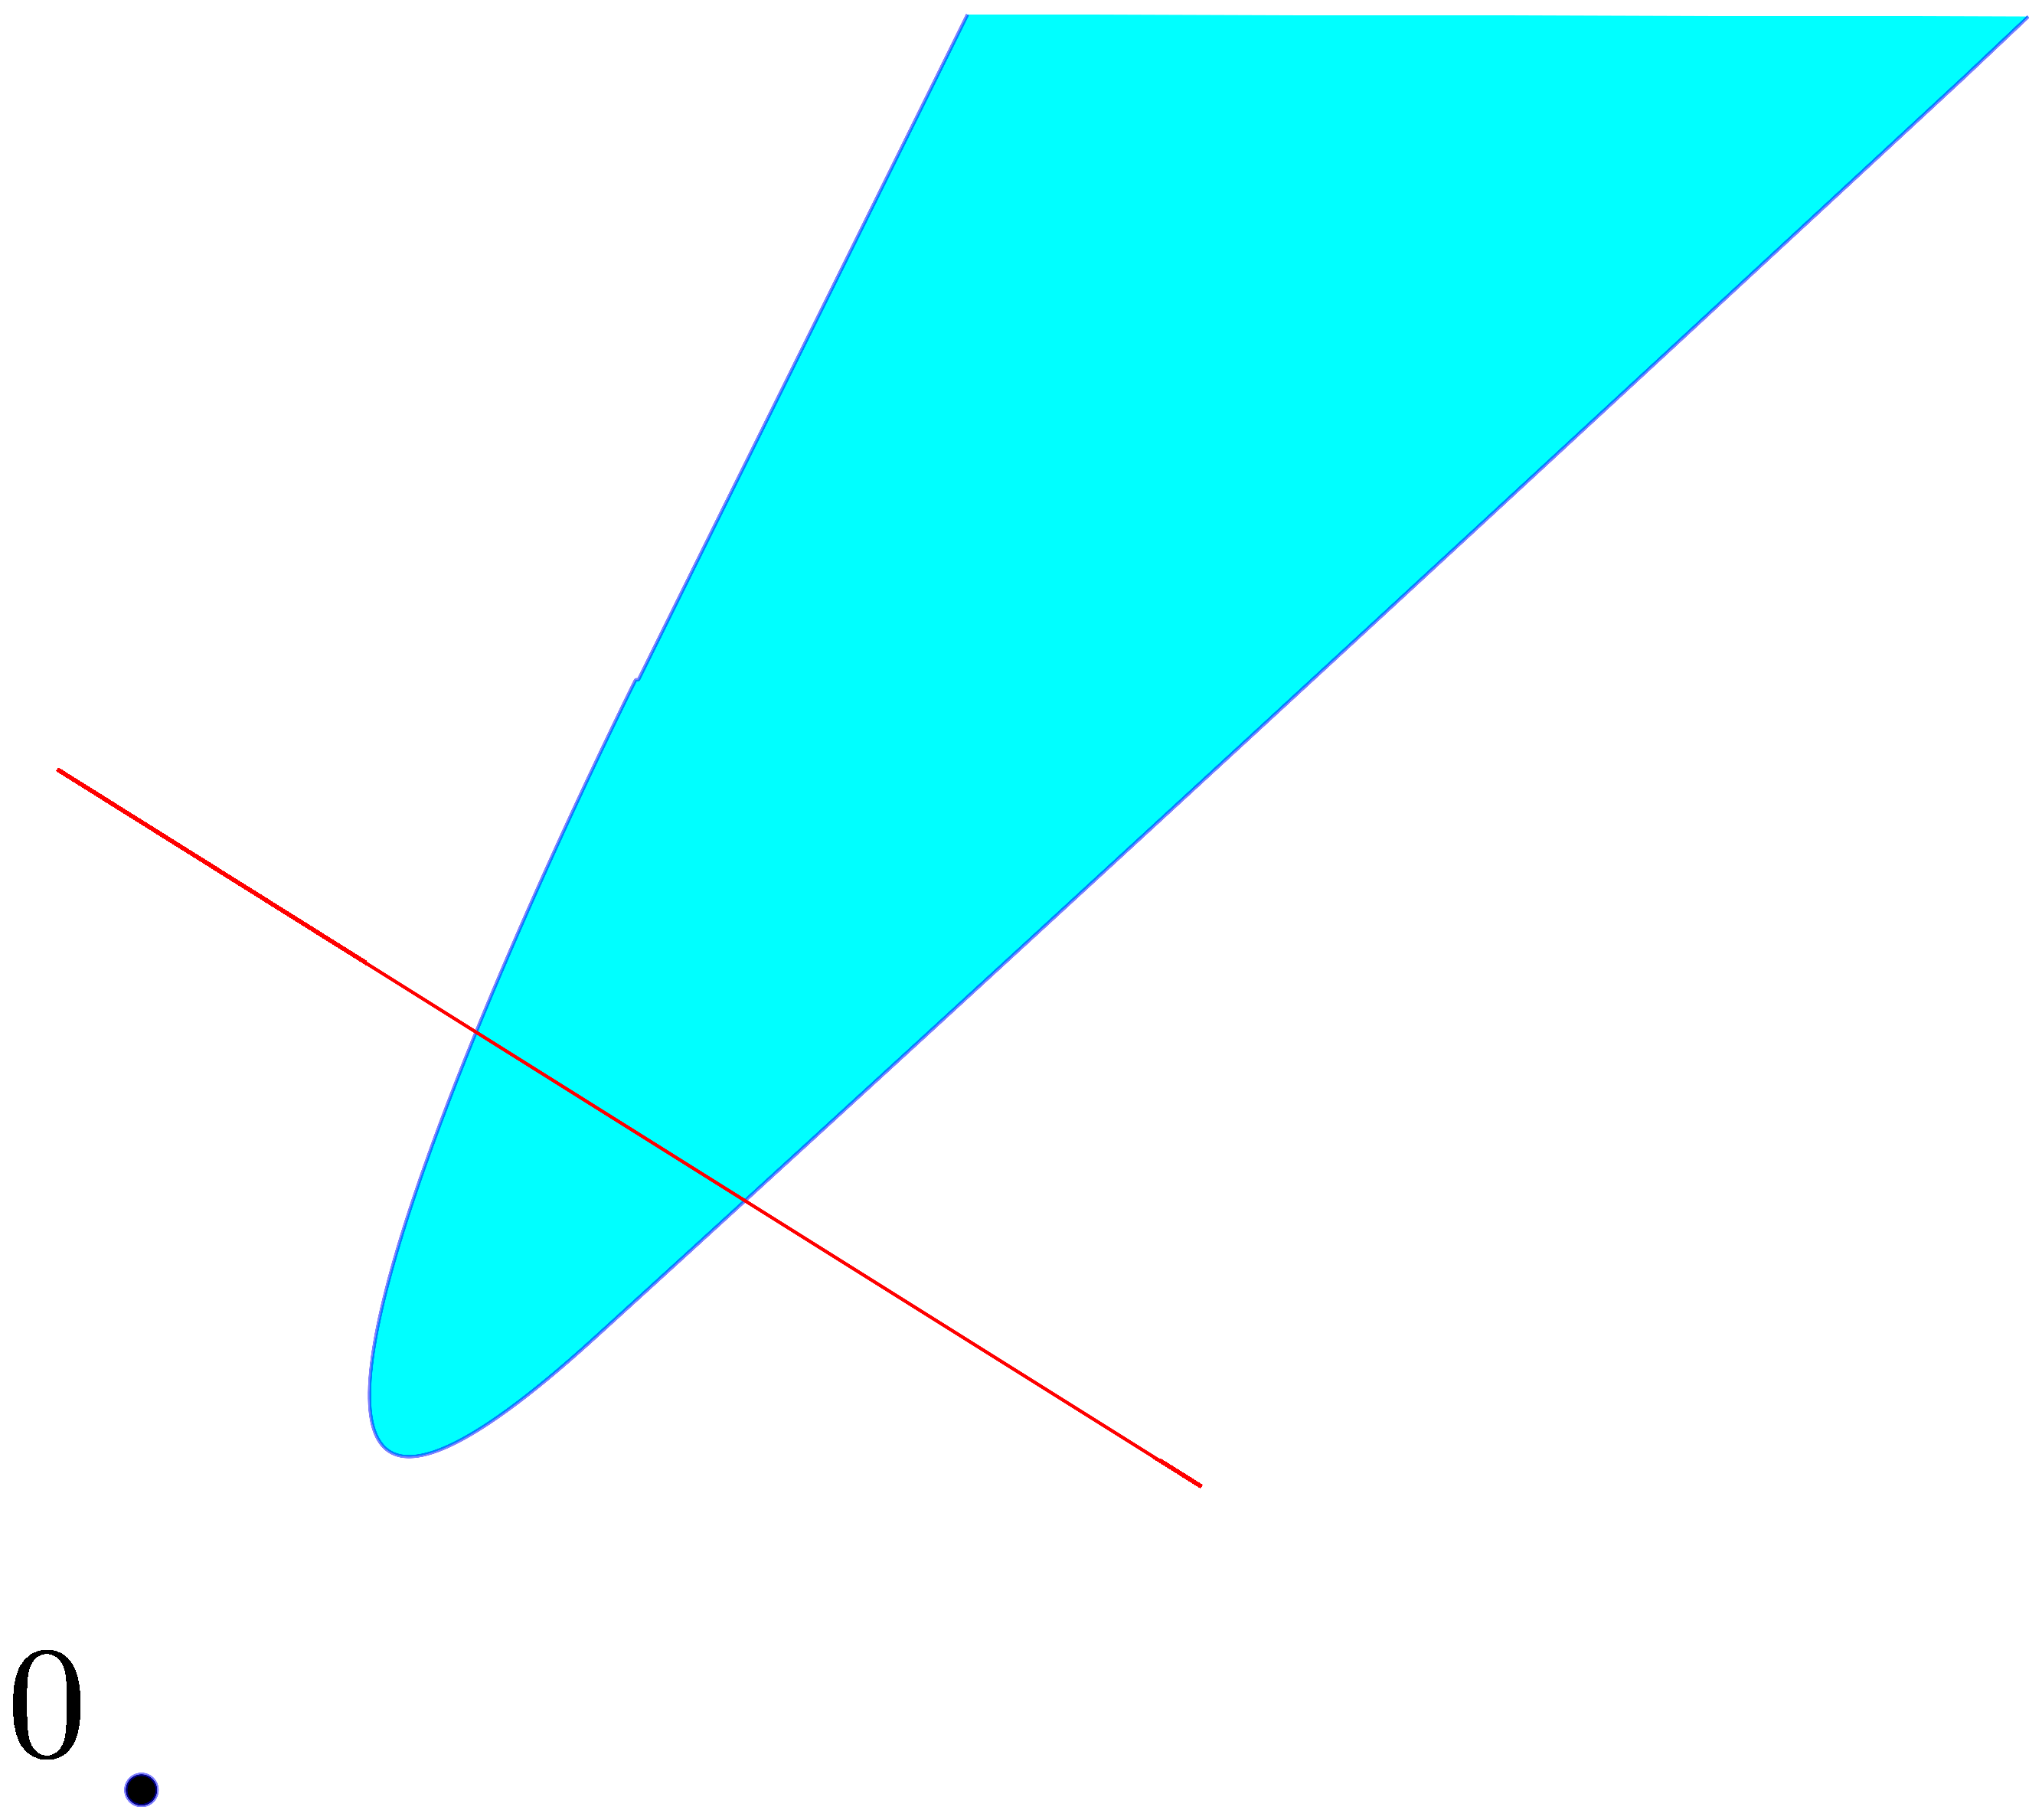
\includegraphics[keepaspectratio, scale=0.095]{figures/asymptotic_meaning_1.eps}
            \end{column}
            \pause
            \begin{column}{0.48\textwidth}
            \centering
            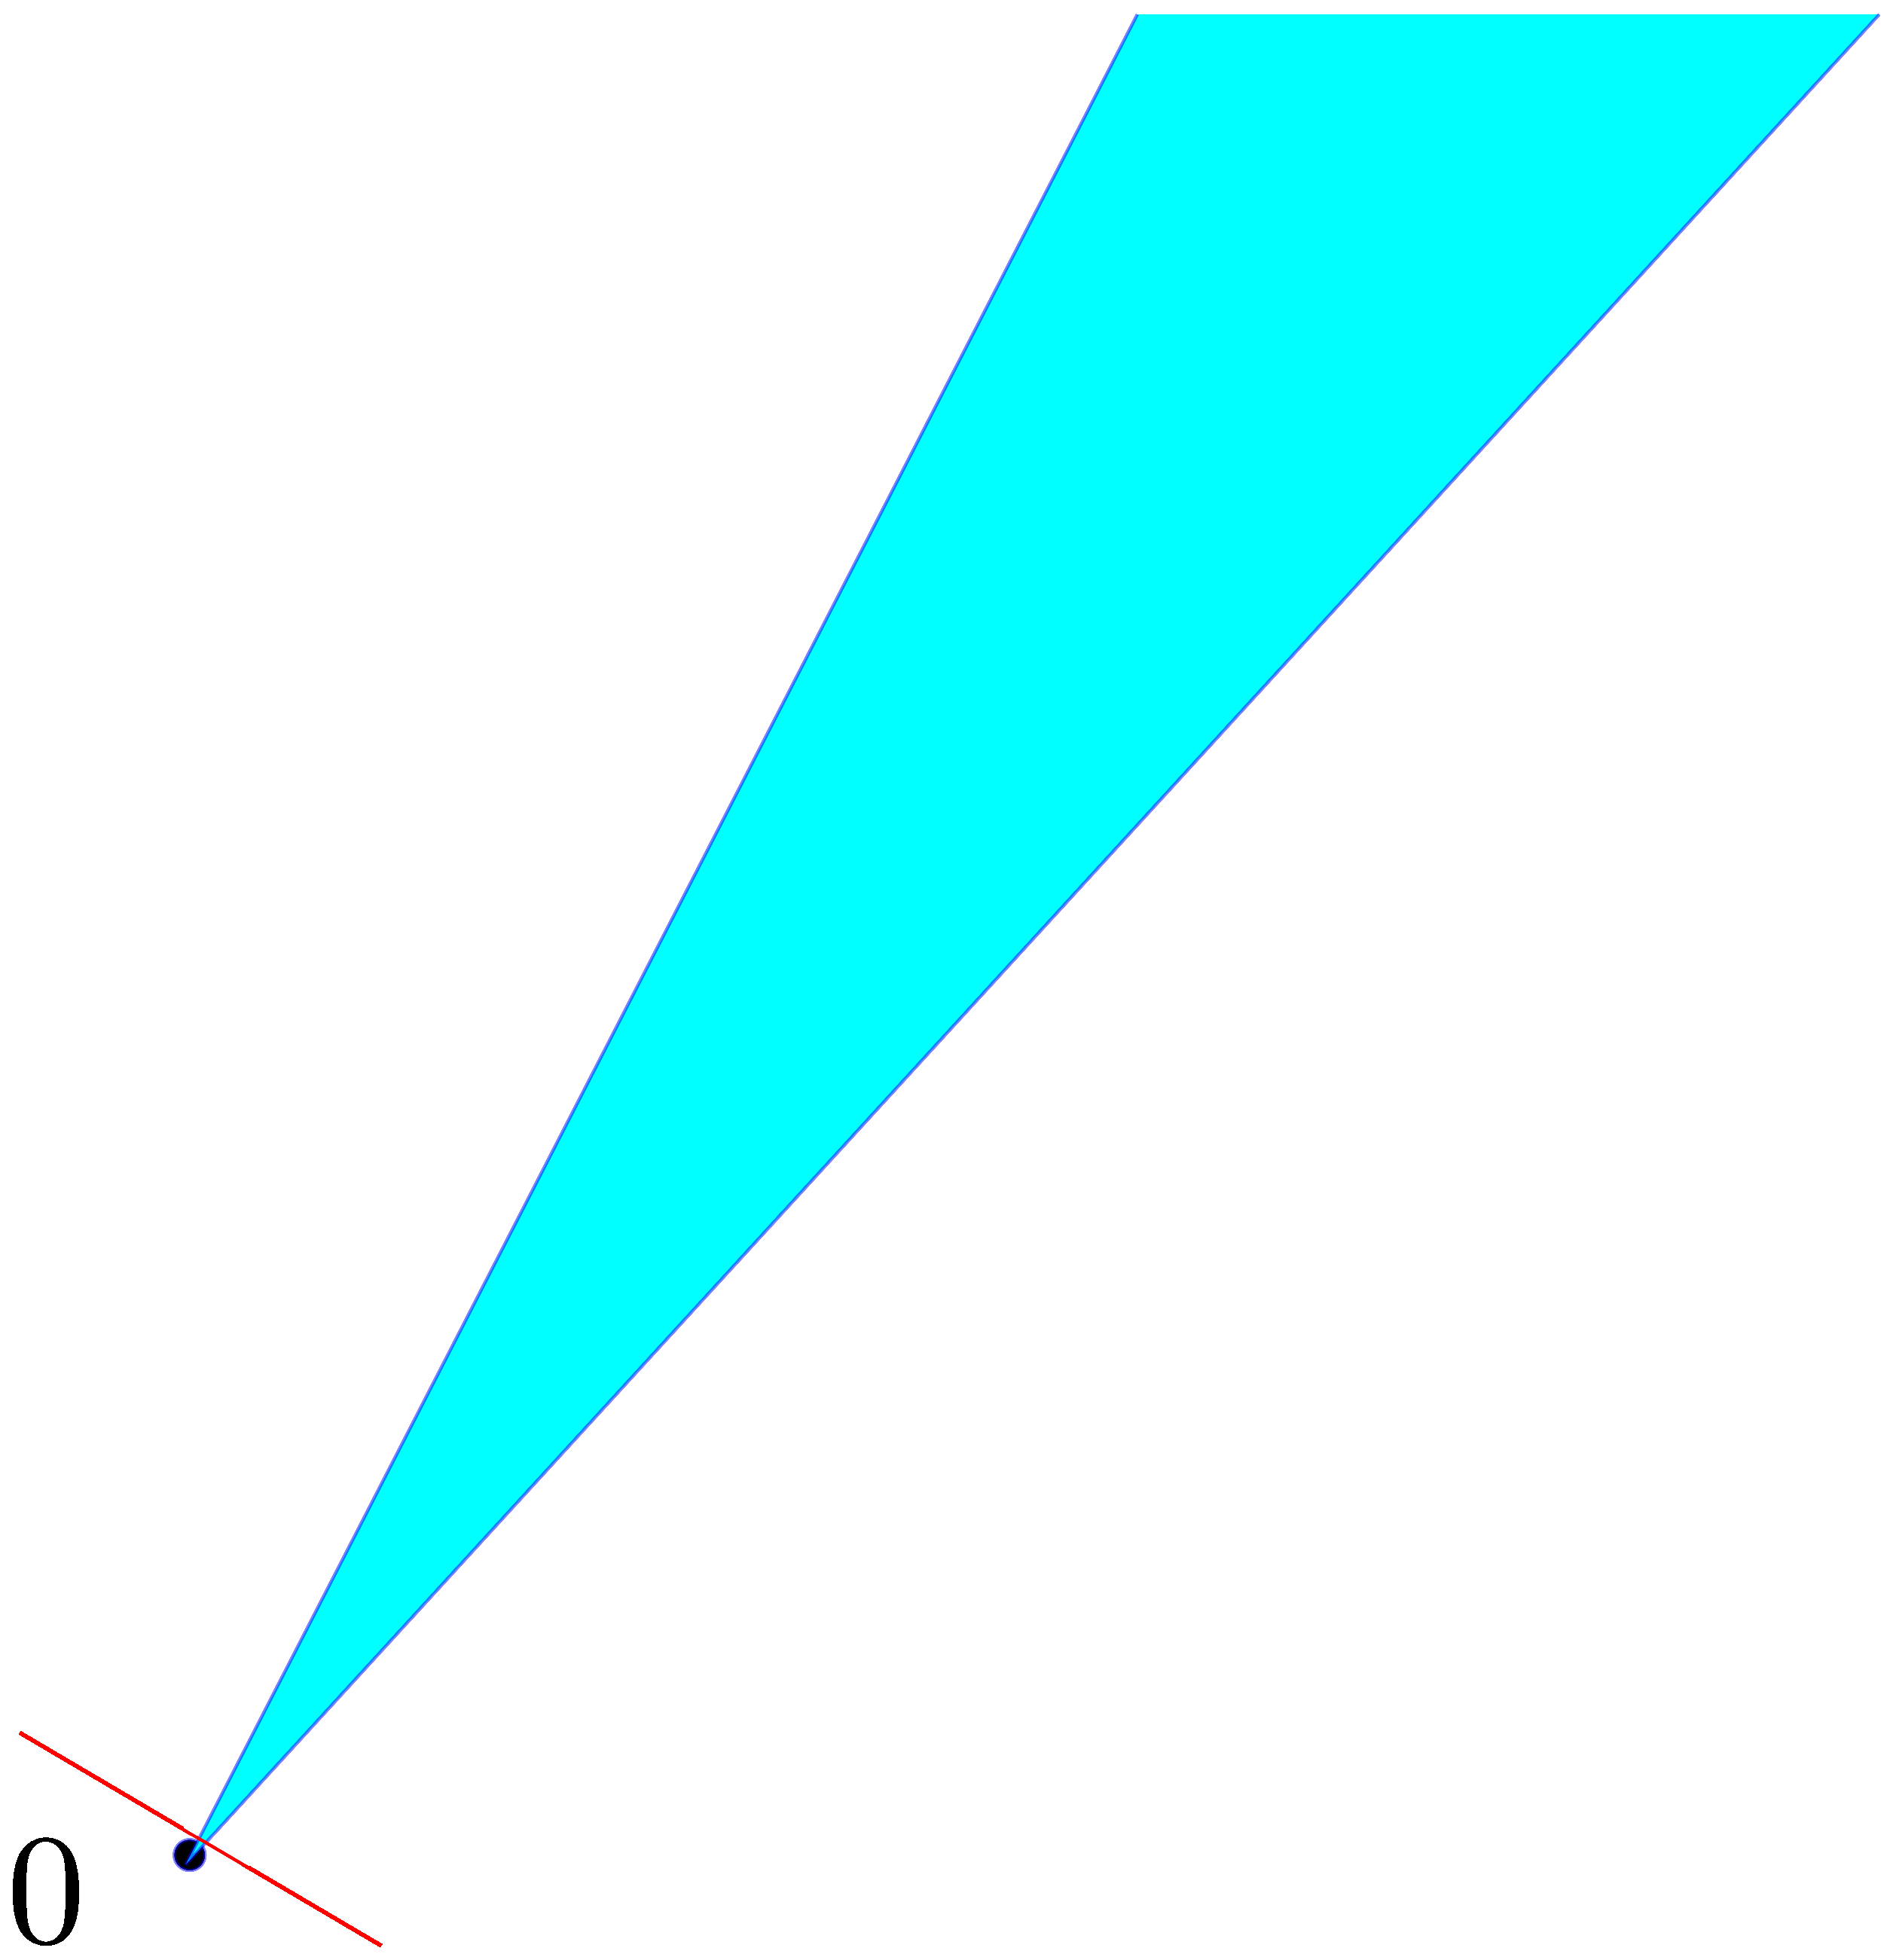
\includegraphics[keepaspectratio, scale=0.095]{figures/asymptotic_meaning_2.eps}
        \end{column}
    \end{columns}
\end{frame}

\begin{frame}{Contents}
    \tableofcontents
\end{frame}

% 1.Preliminary
% ----------------------------------------------------------------
\section{Preliminary}
\begin{frame}{Contents}
    \tableofcontents[currentsection]
\end{frame}

% 1.1
\begin{frame}{Preliminary}
$\NDemenstionalRealEuclideanSpace$: $n$-dimensional real Euclidean space.

The inner product of $\NDemenstionalRealEuclideanSpace$ $\left\langle \cdot ,\cdot \right\rangle$  is defined by

\begin{equation}
    \left\langle x,y\right\rangle \coloneqq \sum_{i = 1}^{n} x_i y_i, \text{for}\: x=(x_1,\dots,x_n)^T \in \mathbb{R}^n \:\text{and}\: y=(y_1,\dots,y_n)^T \in \mathbb{R}^n. \notag
\end{equation}

The norm is defined by $\left\lVert x \right\rVert \coloneqq \left\langle x,x\right\rangle ^{1/2} $.

\end{frame}

% 2.Asymptotic Cones
% ----------------------------------------------------------------
\section{Asymptotic Cones}
\begin{frame}{Contents}
    \tableofcontents[currentsection]
\end{frame}

% 2.1
\begin{frame}{Motivation for Asymptotic Cones}
    Regarding asymptotic cones, we recall the concept of cluster points for bounded sets.

    \begin{block}{Definition 1 (cluster point)}
    $x$ is a cluster point of $\{ x_k \}$ if some subsequence converges to $x$.
    \end{block}

    \begin{block}{Proposition 1}
    The following statements are equivalent:

    \begin{enumerate}[i]
        \item a sequence in $\NDemenstionalRealEuclideanSpace$ converges to $x$,
        \item a sequence is bounded and has $x$ as its unique cluster point.
    \end{enumerate}
    \end{block}

    Generally, we need to consider the uniqueness of cluster point and the boundedness of the given sequence to determine the convergent point in $\NDemenstionalRealEuclideanSpace$.
\end{frame}

% 2.2
\begin{frame}{Motivation for Asymptotic Cones}
    \begin{alertblock}{Remark}
        If the given sequence is bounded, Bolzano-Weierstrass theorem implies that there exists a subsequence which converges to a point.
    \end{alertblock}

    \pause
    How do we consider the convergence of a sequence, which is not bounded?

    Example: $C = \{(x,y) \in \mathbb{R}^2 \:|\: y=x^2\}$

    \centering
    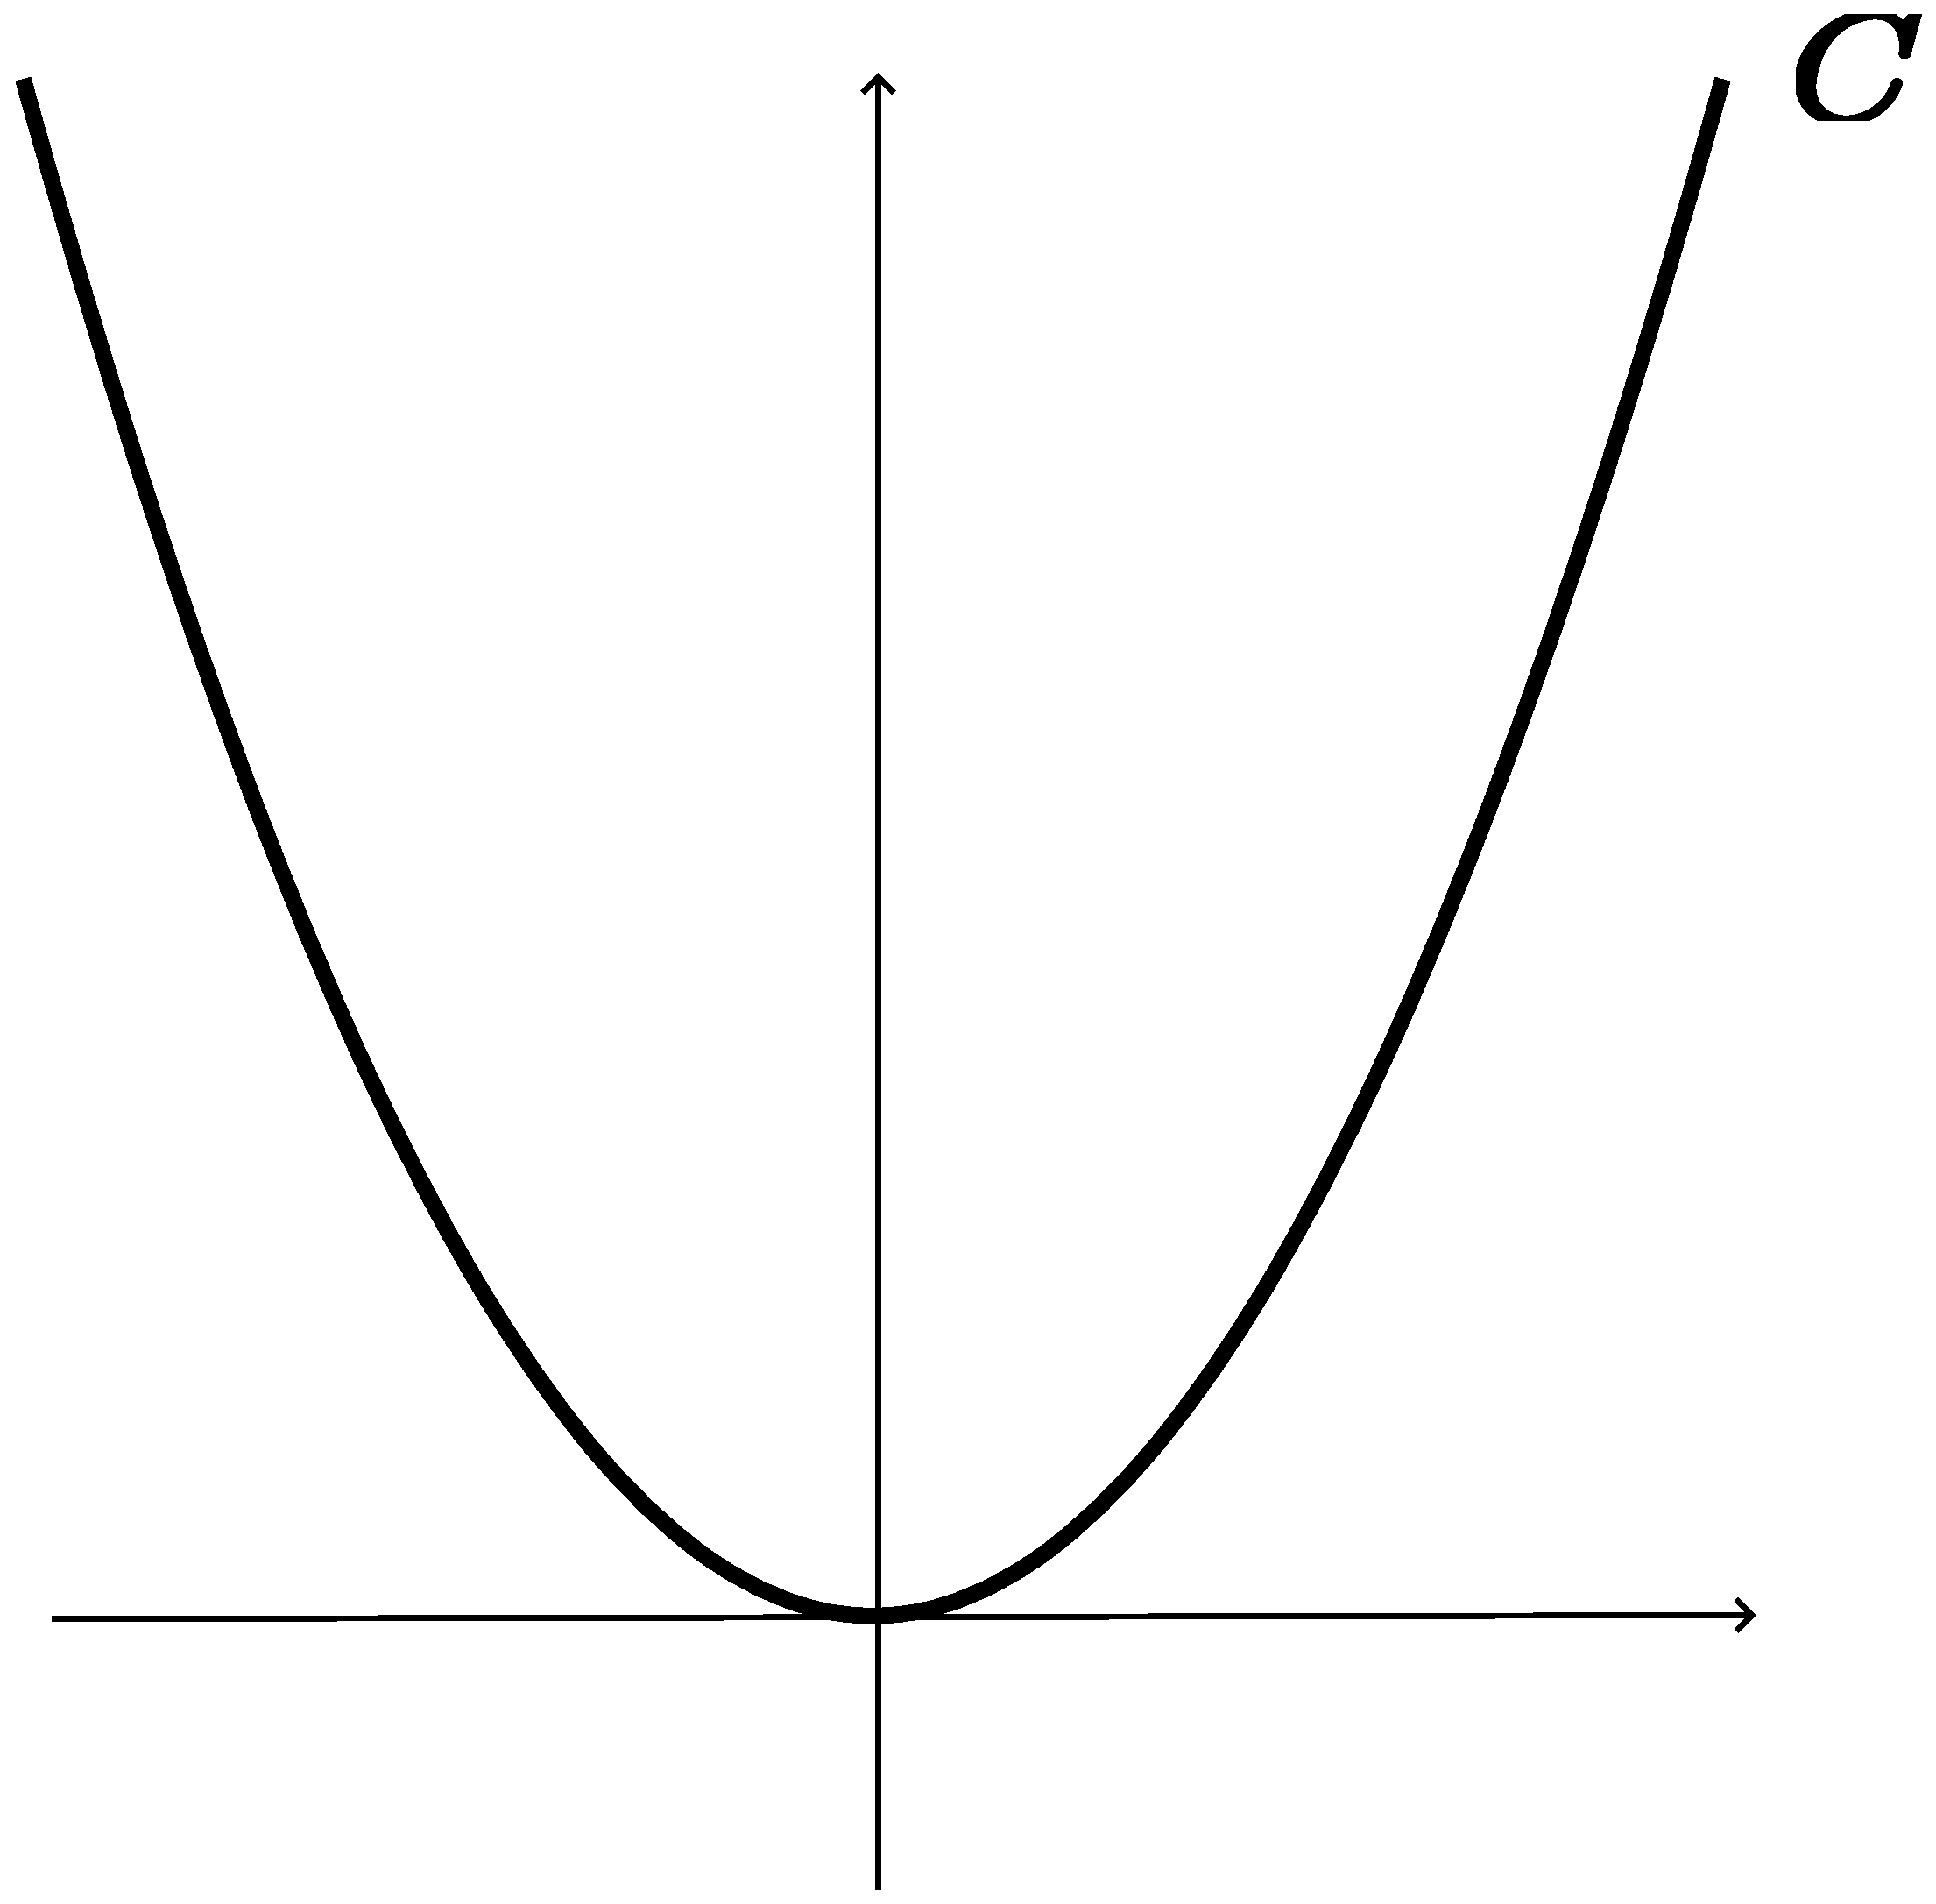
\includegraphics[keepaspectratio, scale=0.10]{figures/figure_quadratic_function.eps}
\end{frame}

% 2.3
\begin{frame}{}
    \begin{block}{Definition 2
        (Asymptotic Cones)}
        $C \subset \mathbb{R}^n$, $C \neq \emptyset$. Then, the asymptotic cone of the set $C$, denoted by $C_\infty$, is the set below with $\{ x_k \} \subset C$;
        \begin{equation}
        C_\infty = \left\{ d \in
        \mathbb{R}^n \:\middle|\: \exists t_k \rightarrow +\infty, \exists x_k \in C \:\text{with}\: \lim_{k \to \infty} \frac{x_k}{t_k} = d \right\}. \notag
        \end{equation}
    \end{block}

    Example: $C = \{(x,y) \in \mathbb{R}^2 \:|\: y=x^2\}$. We let $\textcolor{blue}{x_k} = (k, k^2)$ and $t_k = \left\lVert x_k \right\rVert$.

    \centering
    \begin{columns}
        \pause
        \begin{column}{0.48\textwidth}
        \centering
        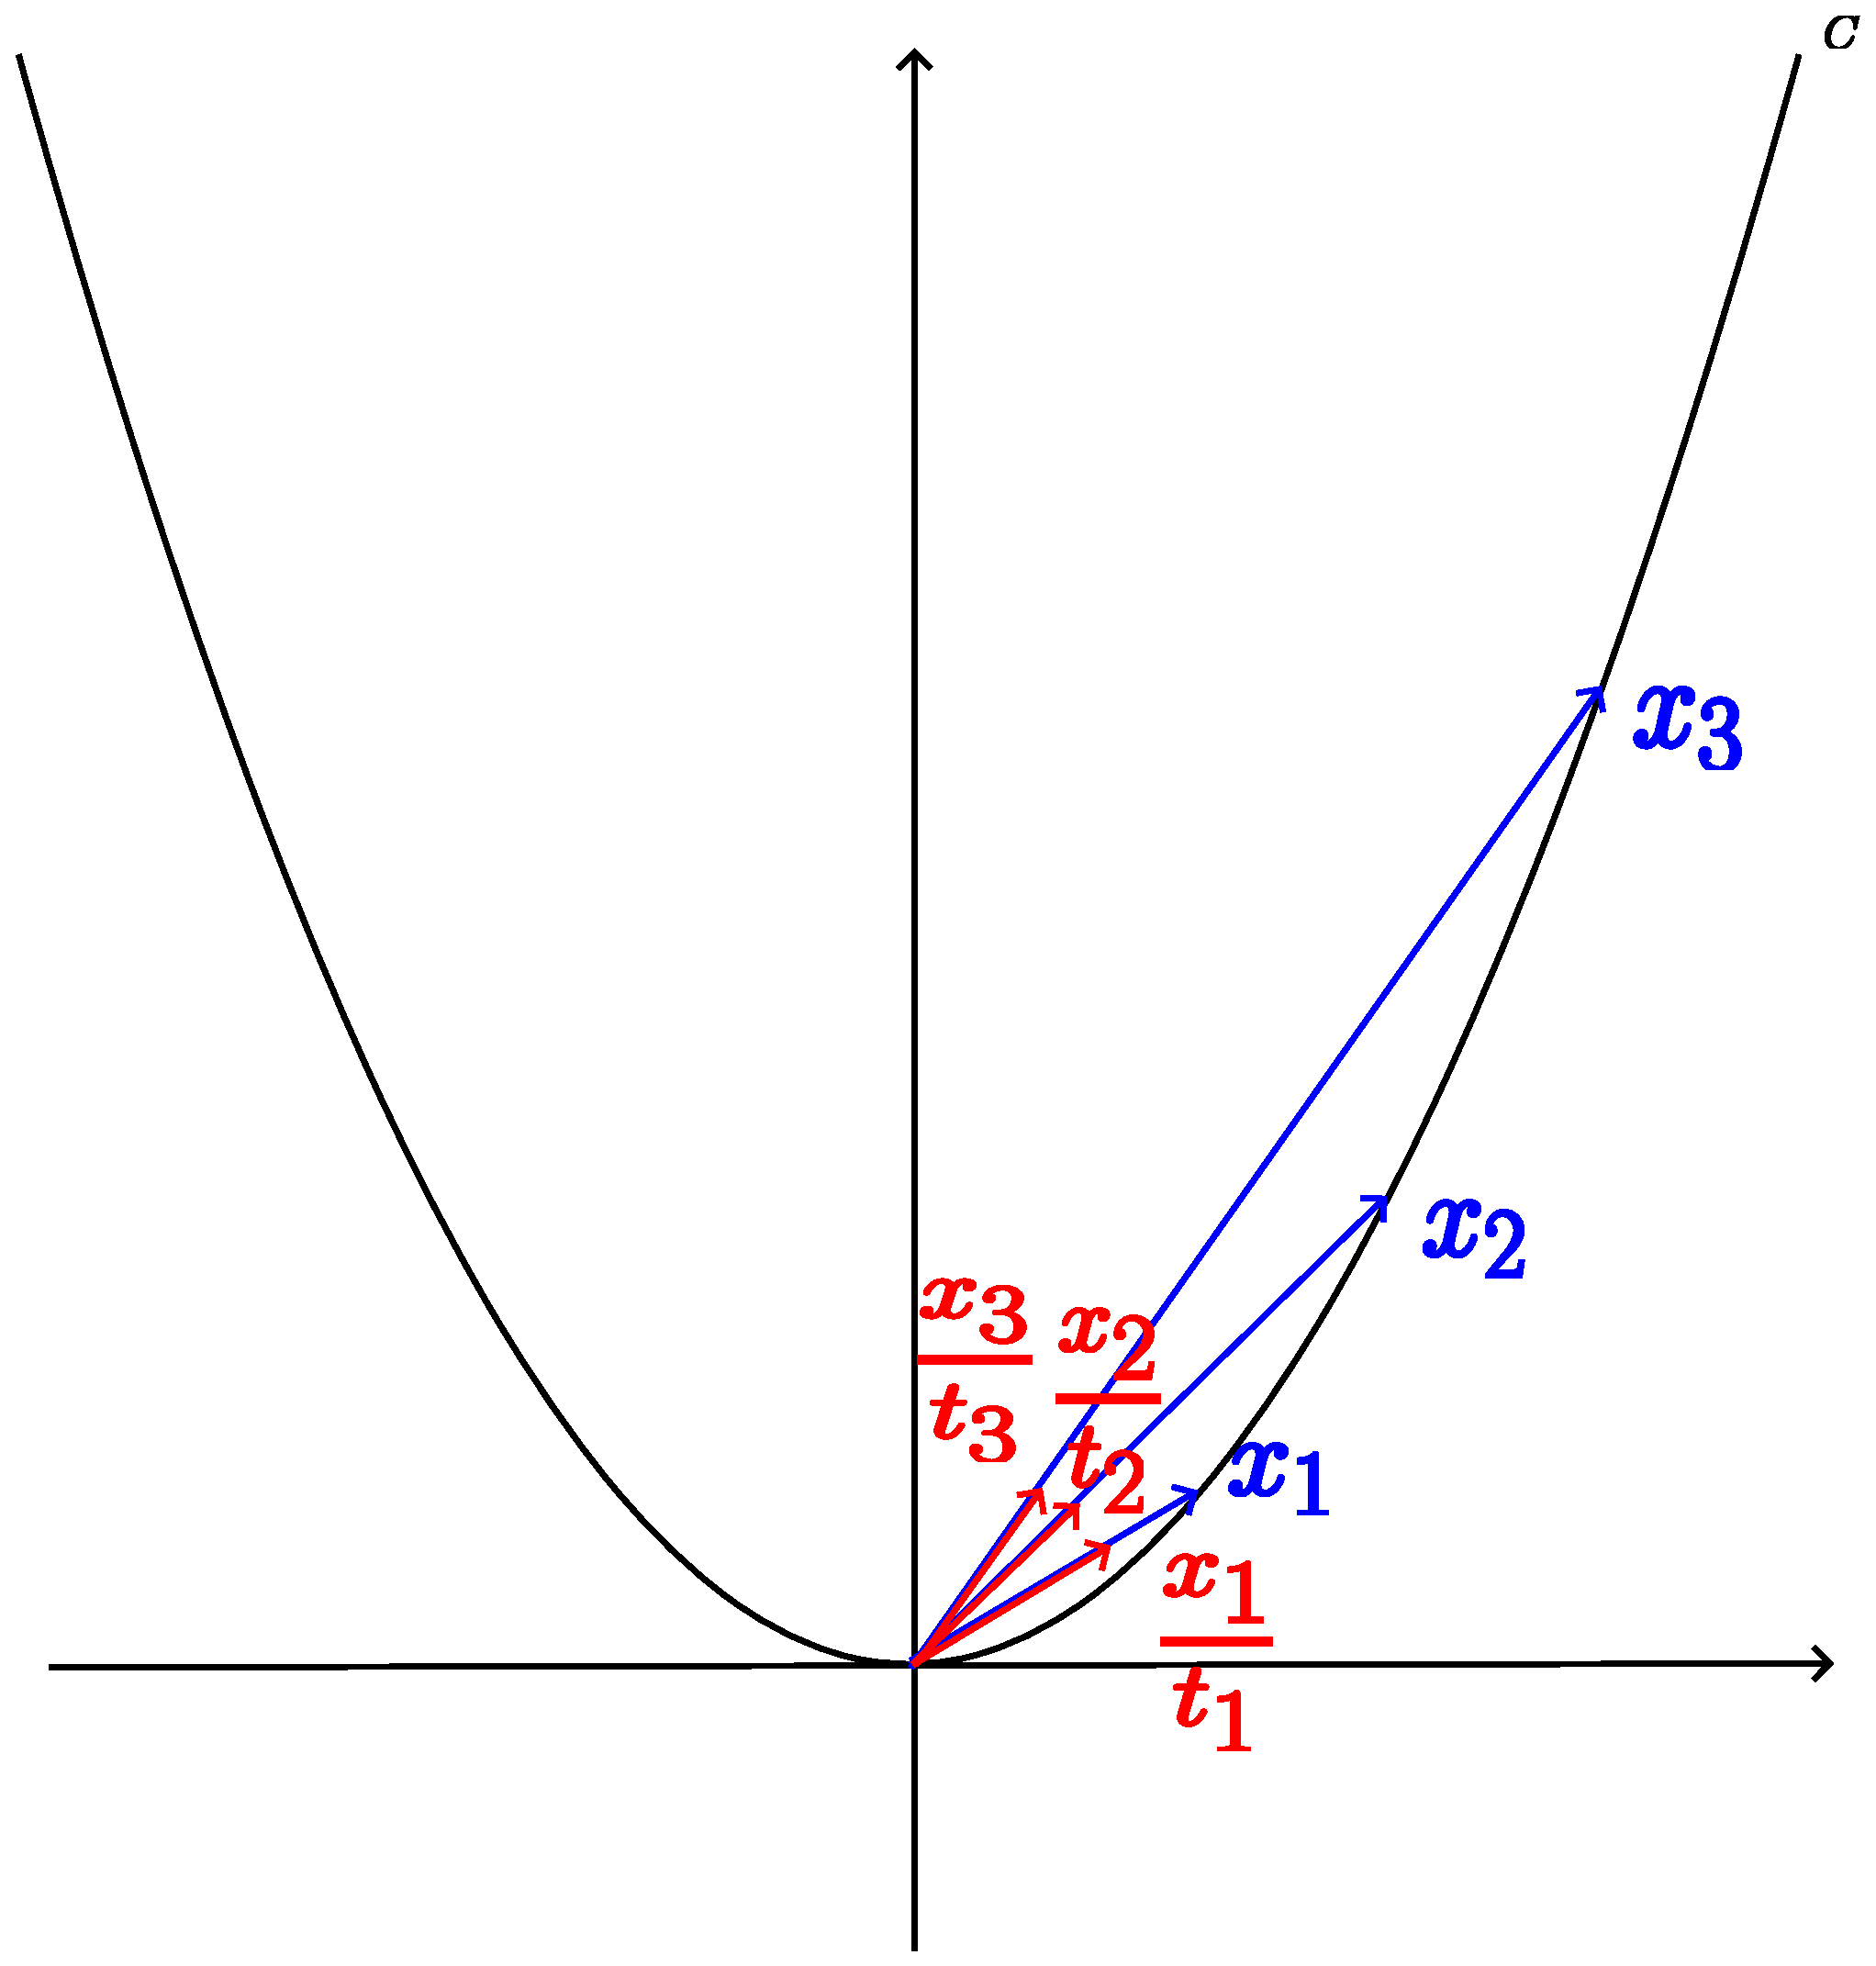
\includegraphics[keepaspectratio, scale=0.095]{figures/figure_asymptotic_cone_1.eps}
        \end{column}
        \pause
        \begin{column}{0.48\textwidth}
        \centering
        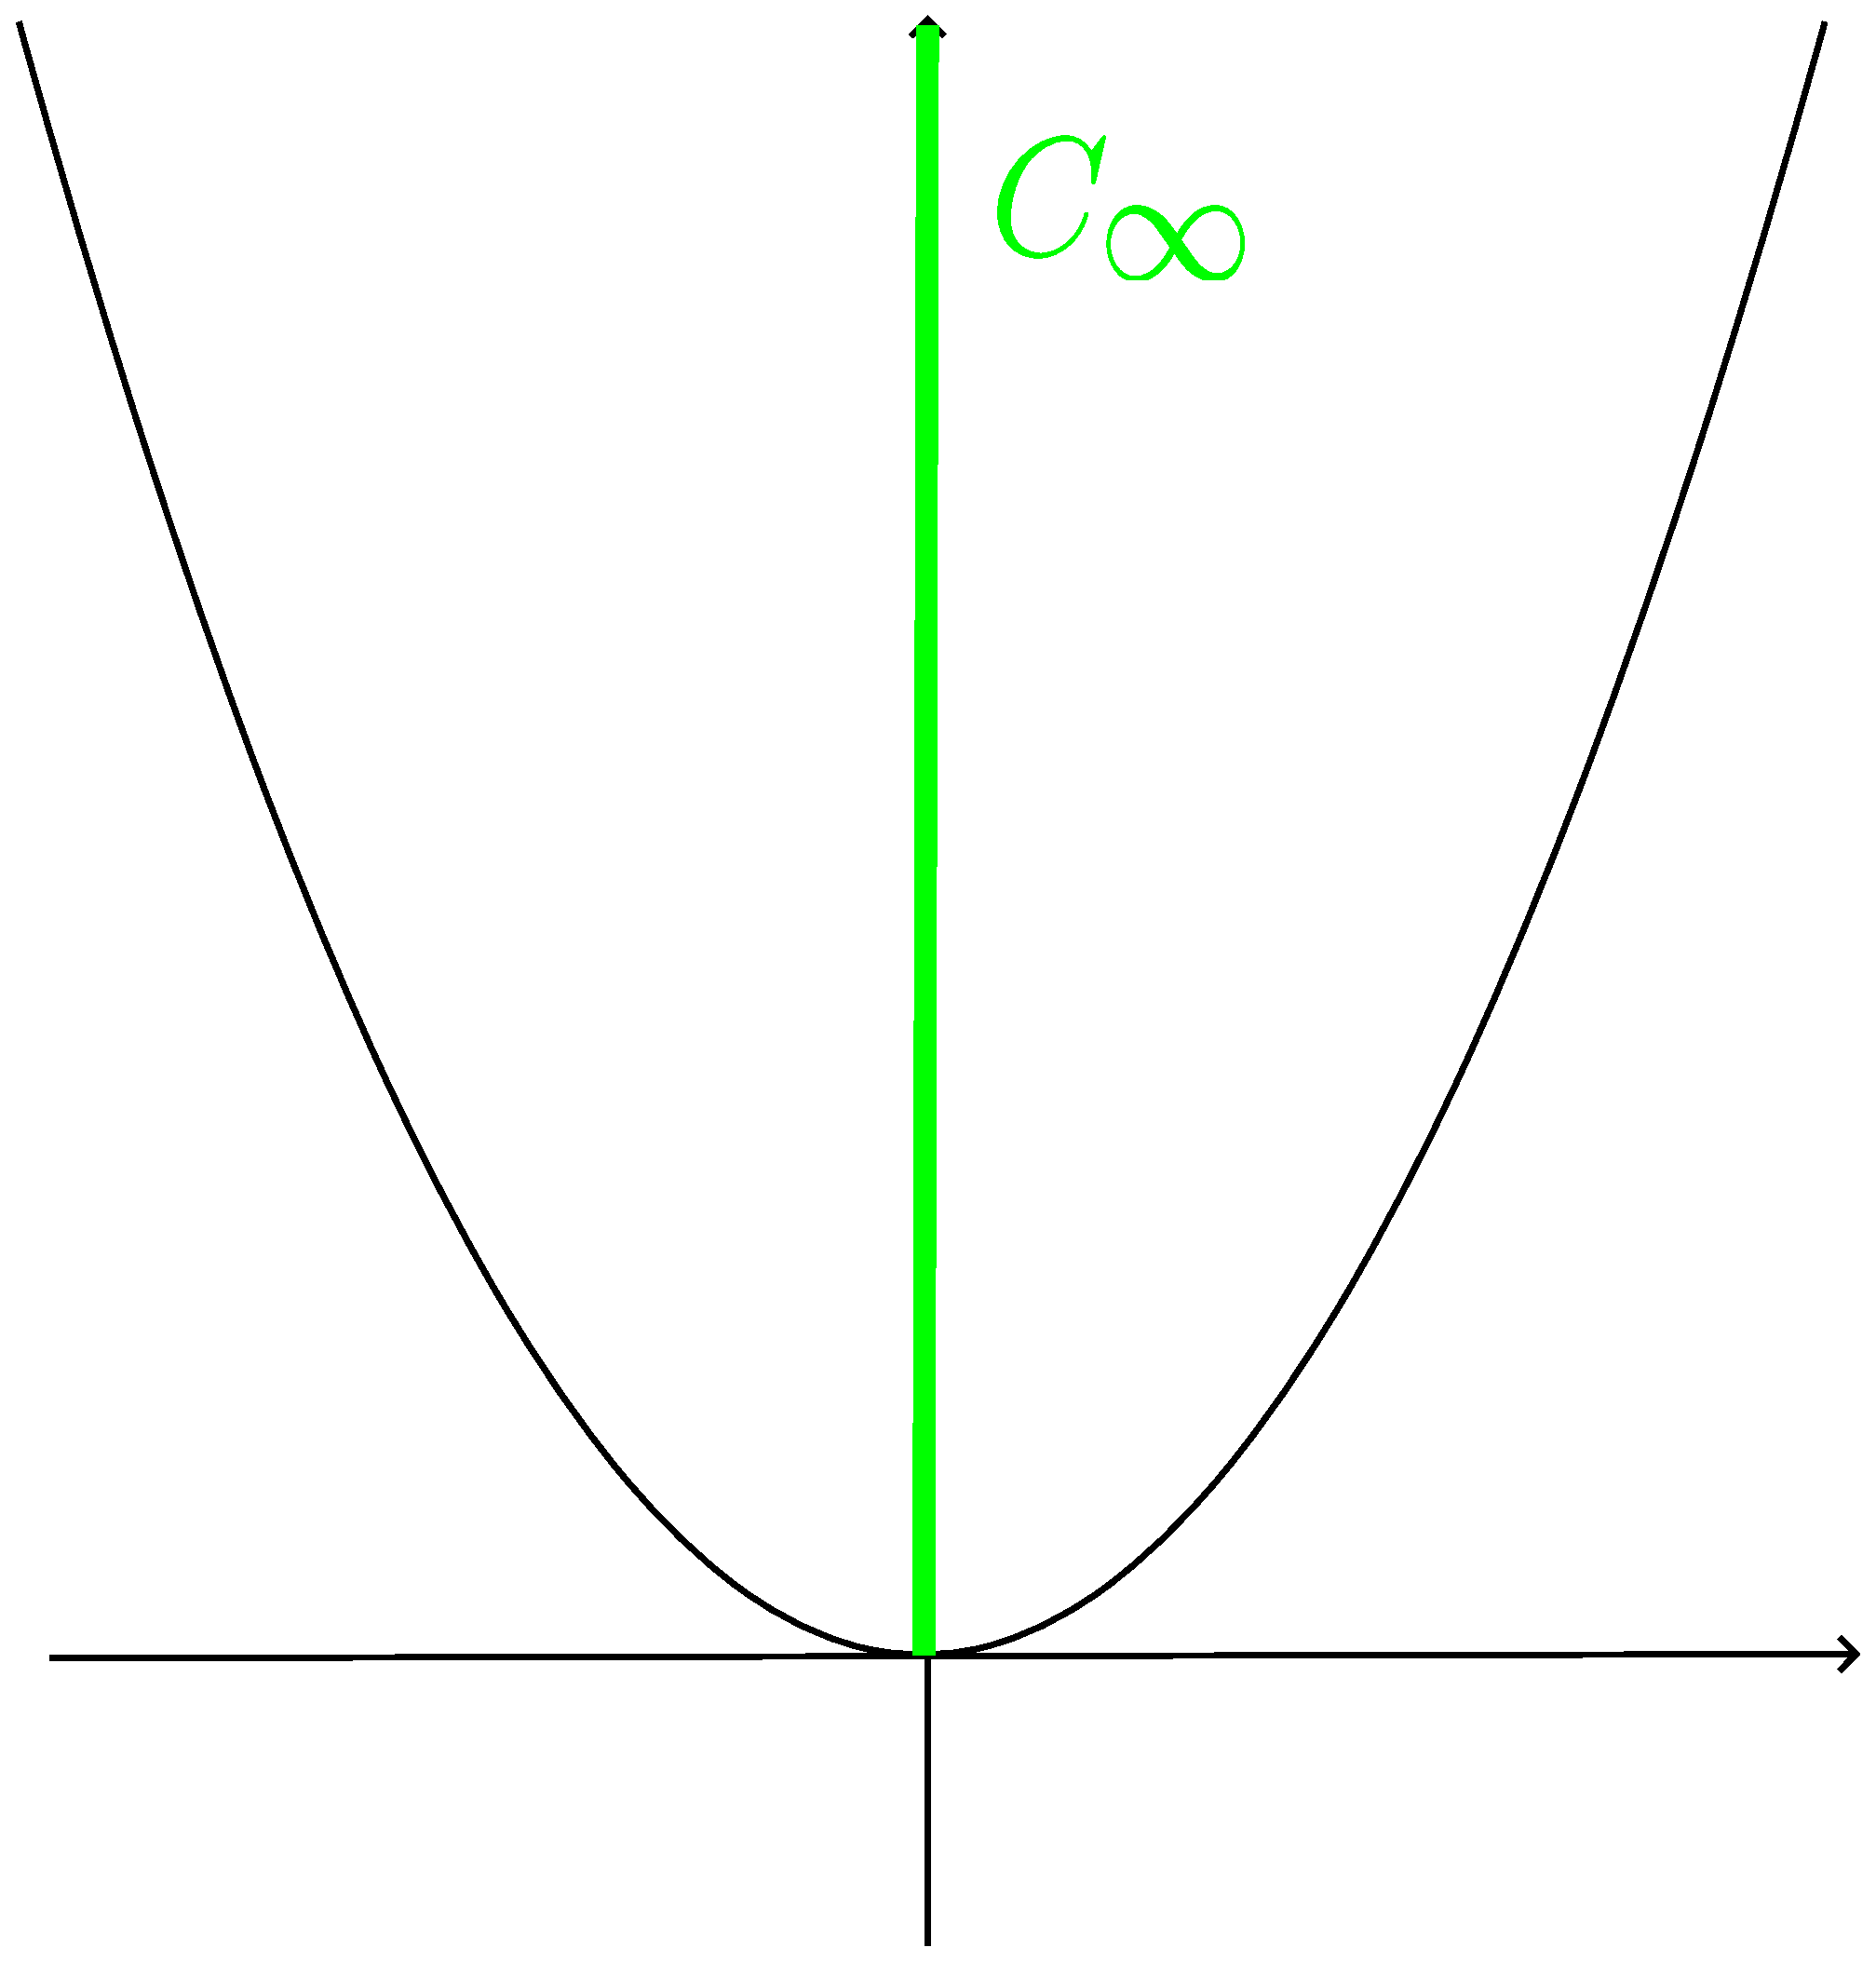
\includegraphics[keepaspectratio, scale=0.095]{figures/figure_asymptotic_cone_2.eps}
        \end{column}
    \end{columns}
\end{frame}


% 2.4
\begin{frame}{Properties around Asymptotic Cones}
    \begin{block}{Proposition 2}
    A set $C \subset \mathbb{R}^n$ is bounded if and only if $C_\infty = \{0\}$.
    \end{block}

    \begin{block}{Definition 3}
    Let $C \subset \NDemenstionalRealEuclideanSpace$ be nonempty and define
    \begin{equation}
        C_{\infty}^1 = \left\{d \in \NDemenstionalRealEuclideanSpace \:\middle|\: \forall t_k \rightarrow + \infty , \exists x_k \in C \:\text{ with }\: \lim_{k \to \infty} \frac{x_k}{t_k} = d \right\}. \notag
    \end{equation}
    We say that $C$ is asymptotically regular if $C_{\infty} = C_{\infty}^1$.
    \end{block}

    \begin{block}{Proposition 3}
    Let $C$ be a nonempty convex set in $\NDemenstionalRealEuclideanSpace$. Then $C$ is asymptotically regular.
    \end{block}
\end{frame}

% 2.5
\begin{frame}{Example of Asymptotically Regular}
    \begin{block}{Definition 3}
        Let $C \subset \NDemenstionalRealEuclideanSpace$ be nonempty and define
        \begin{equation}
            C_{\infty}^1 = \left\{d \in \NDemenstionalRealEuclideanSpace \:\middle|\: \forall t_k \rightarrow + \infty , \exists x_k \in C \:\text{ with }\: \lim_{k \to \infty} \frac{x_k}{t_k} = d \right\}. \notag
        \end{equation}
        We say that $C$ is asymptotically regular if $C_{\infty} = C_{\infty}^1$.
    \end{block}

    Example: $D$ is NOT asymptotically regular.

    \centering
    \begin{columns}
        \begin{column}{0.48\textwidth}
        \centering
        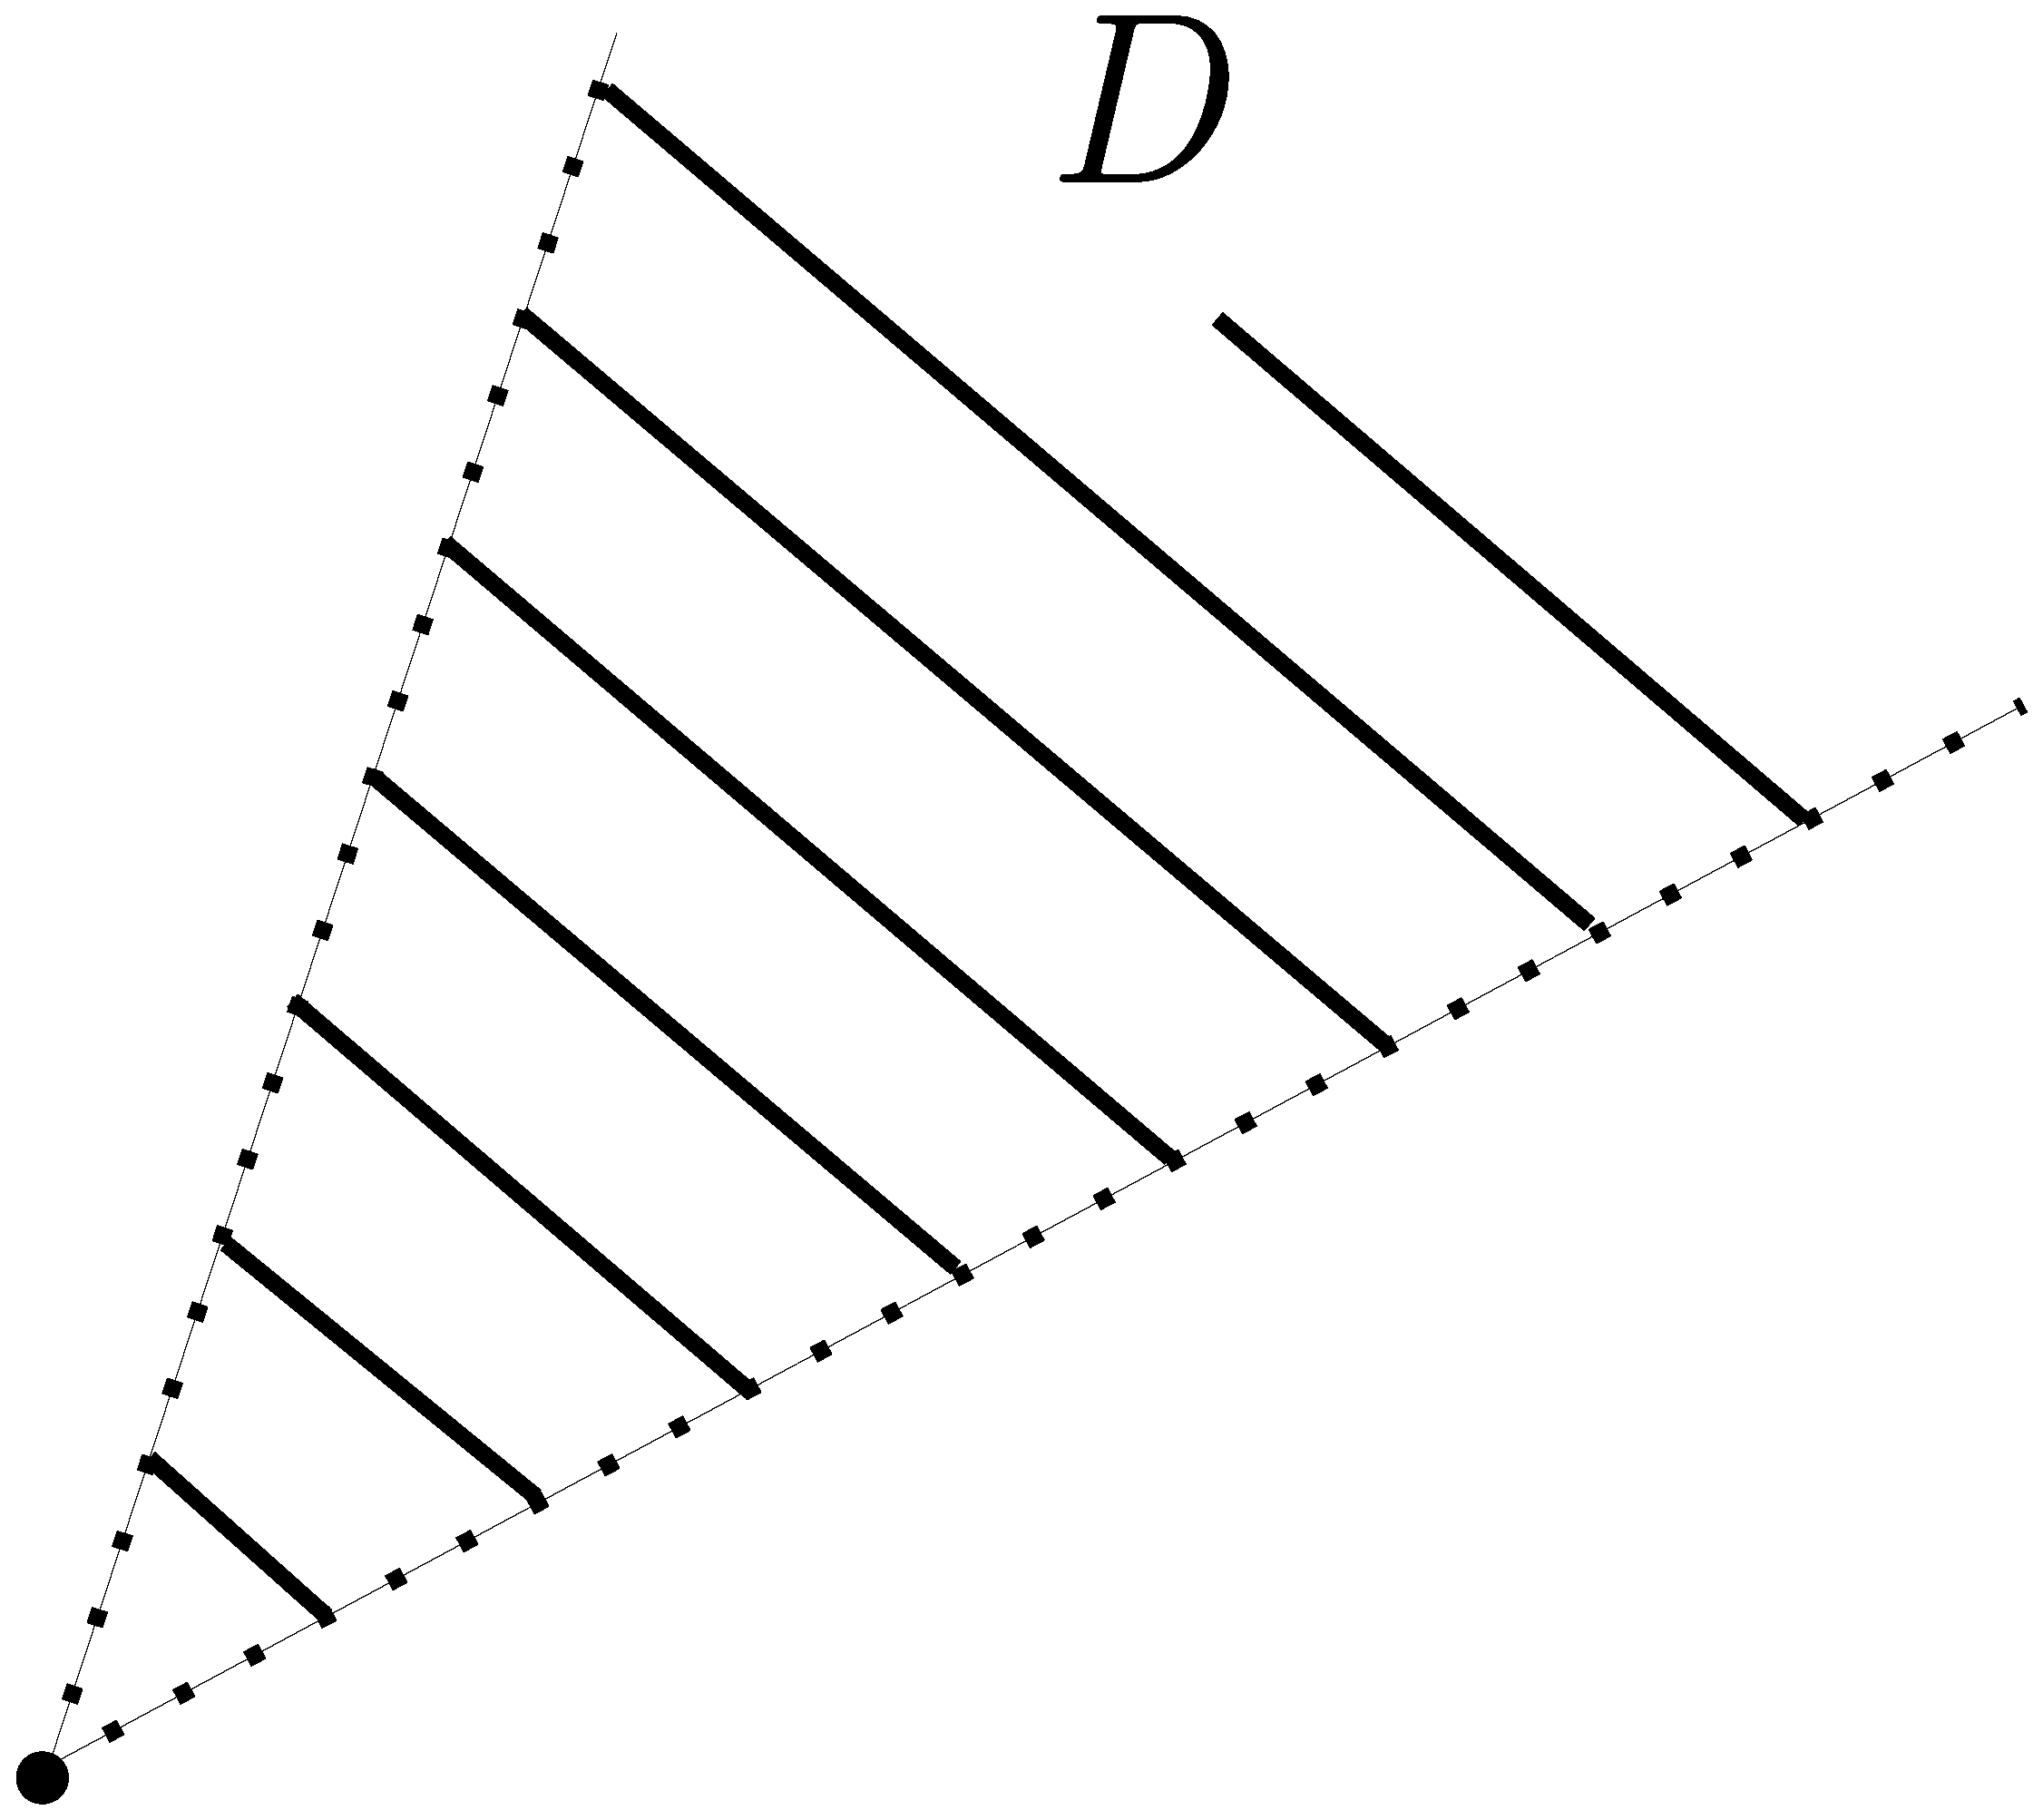
\includegraphics[keepaspectratio, scale=0.085]{figures/example_not_asymptotically_regular_1.eps}
        \end{column}
        \pause
        \begin{column}{0.48\textwidth}
        \centering
        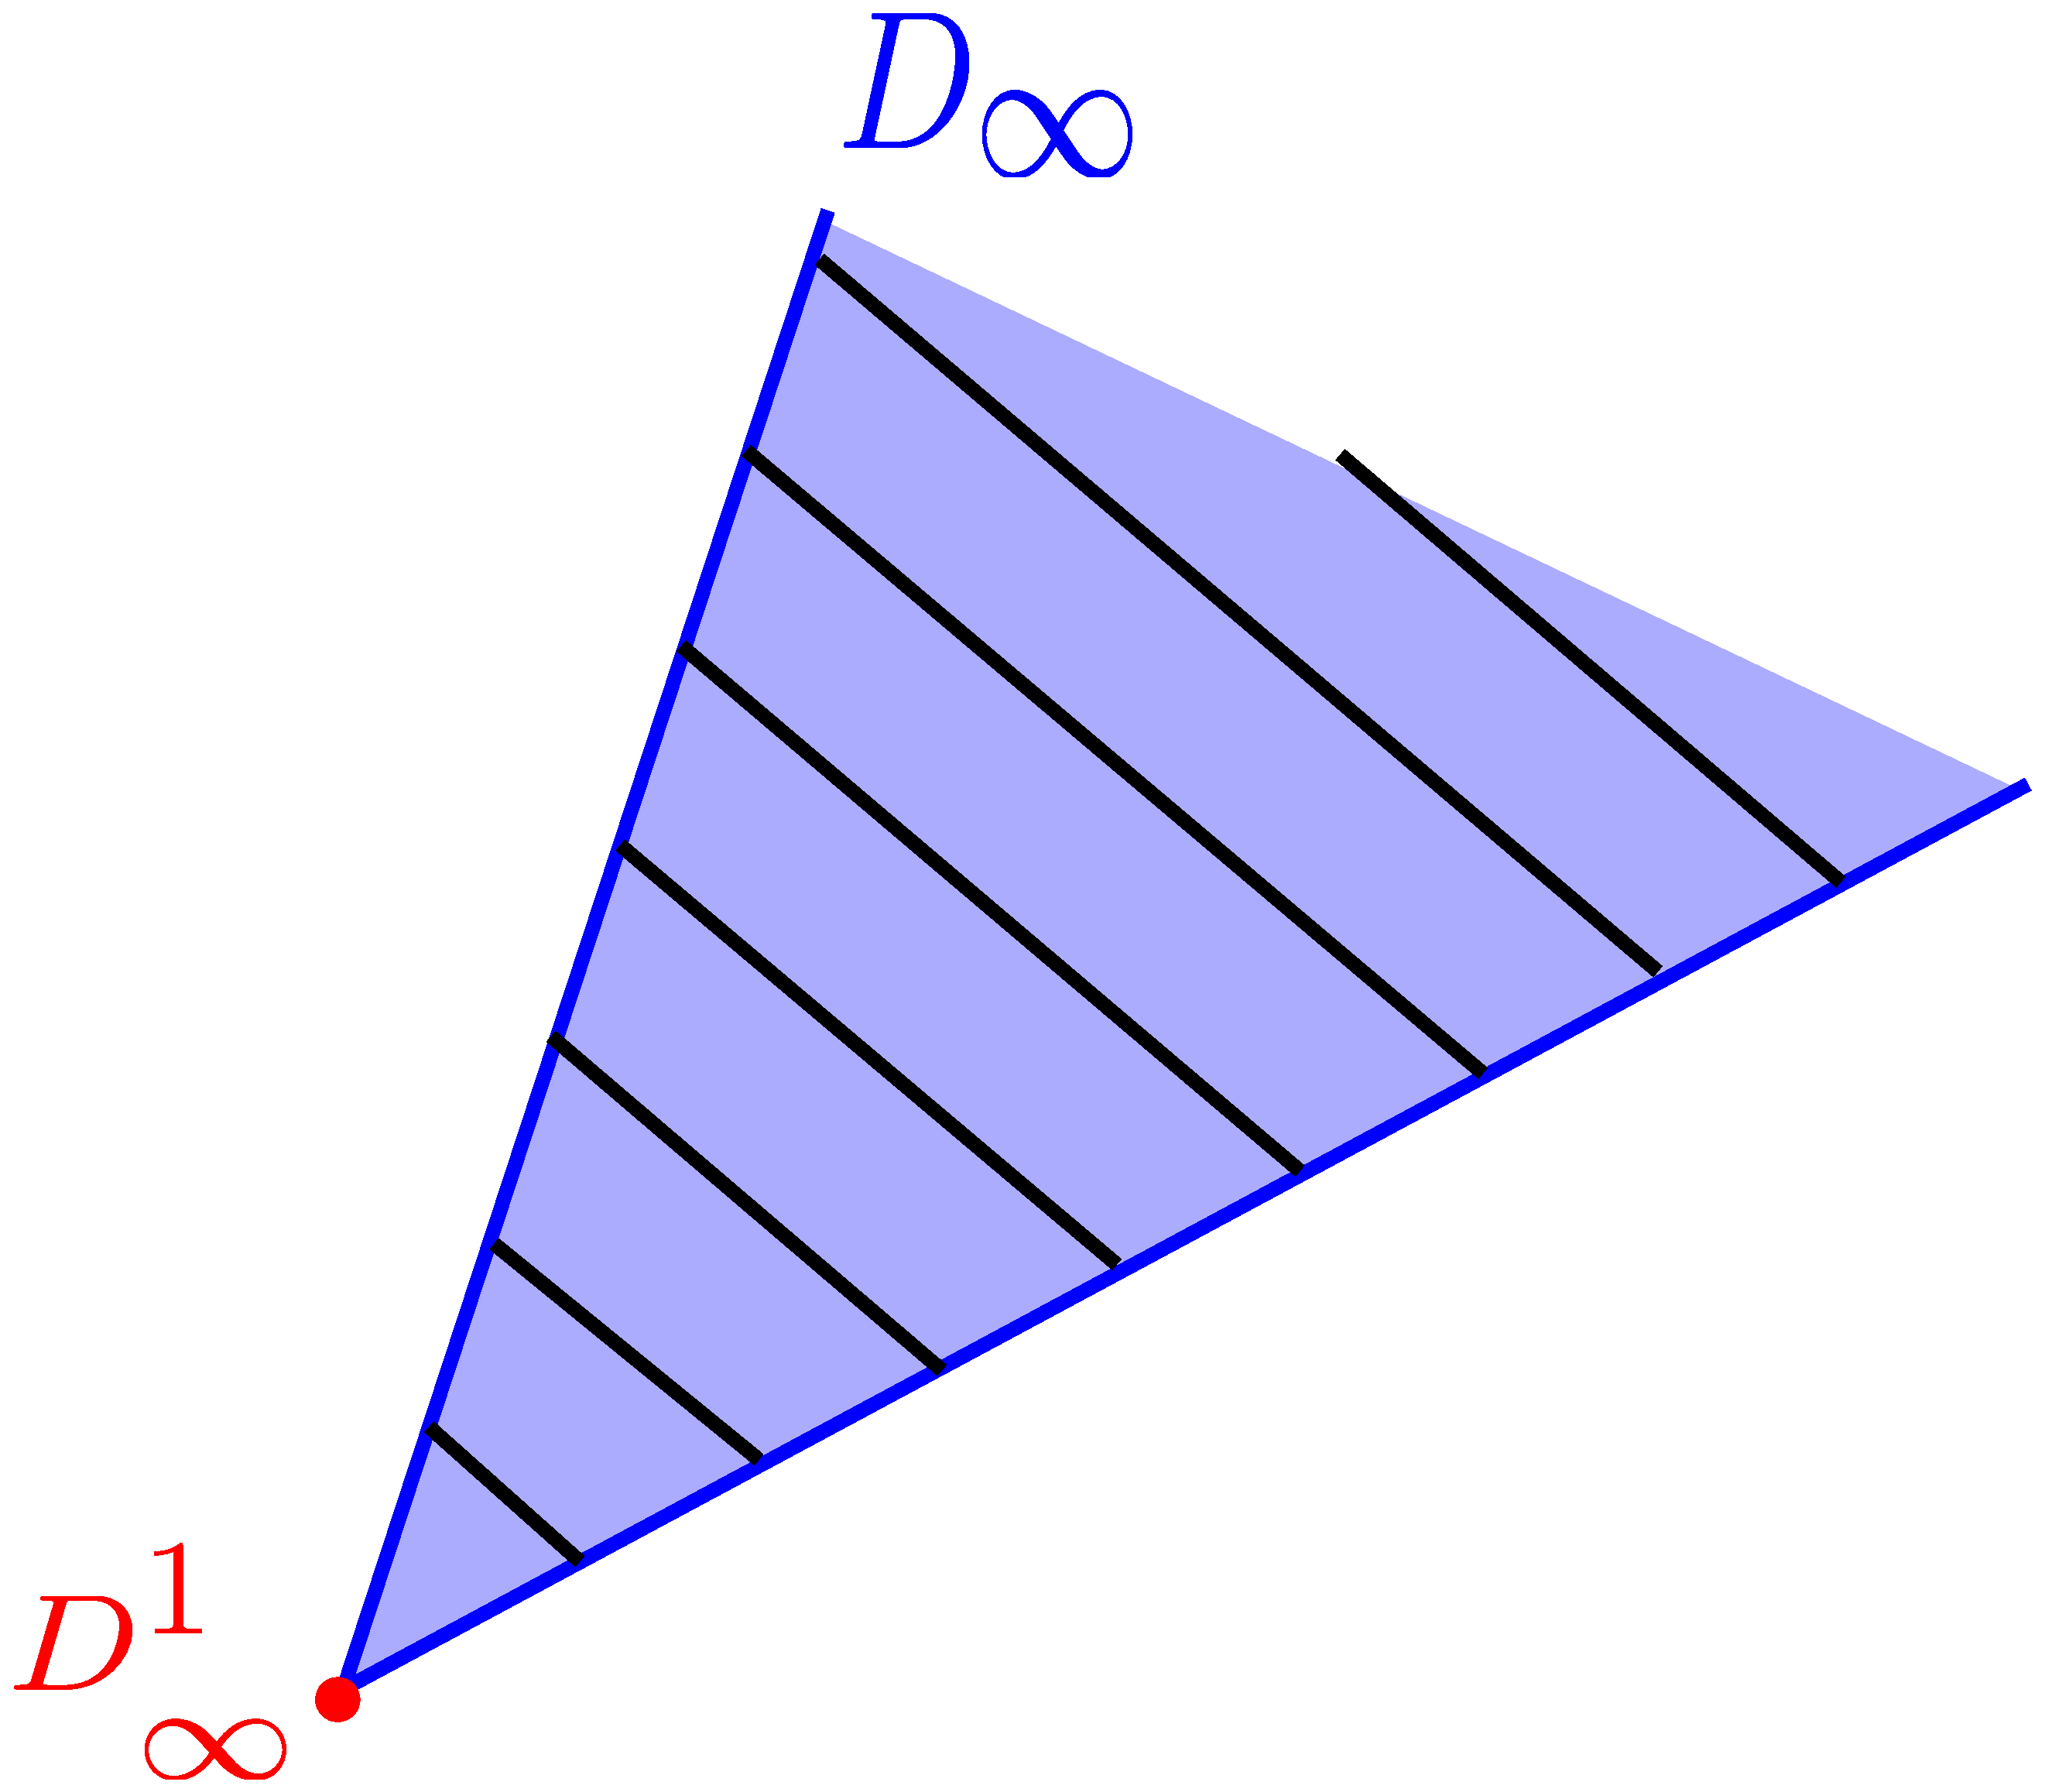
\includegraphics[keepaspectratio, scale=0.085]{figures/example_not_asymptotically_regular_2.eps}
        \end{column}
    \end{columns}
\end{frame}

% 2.6
\begin{frame}{Example of Asymptotically Regular}
    \begin{block}{Proposition 3}
        Let $C$ be a nonempty convex set in $\NDemenstionalRealEuclideanSpace$. Then $C$ is asymptotically regular.
    \end{block}

    Example: $E$ is not convex but $E$ is asymptotically regular.

    \medskip

    \centering
    \begin{columns}
        \begin{column}{0.48\textwidth}
        \centering
        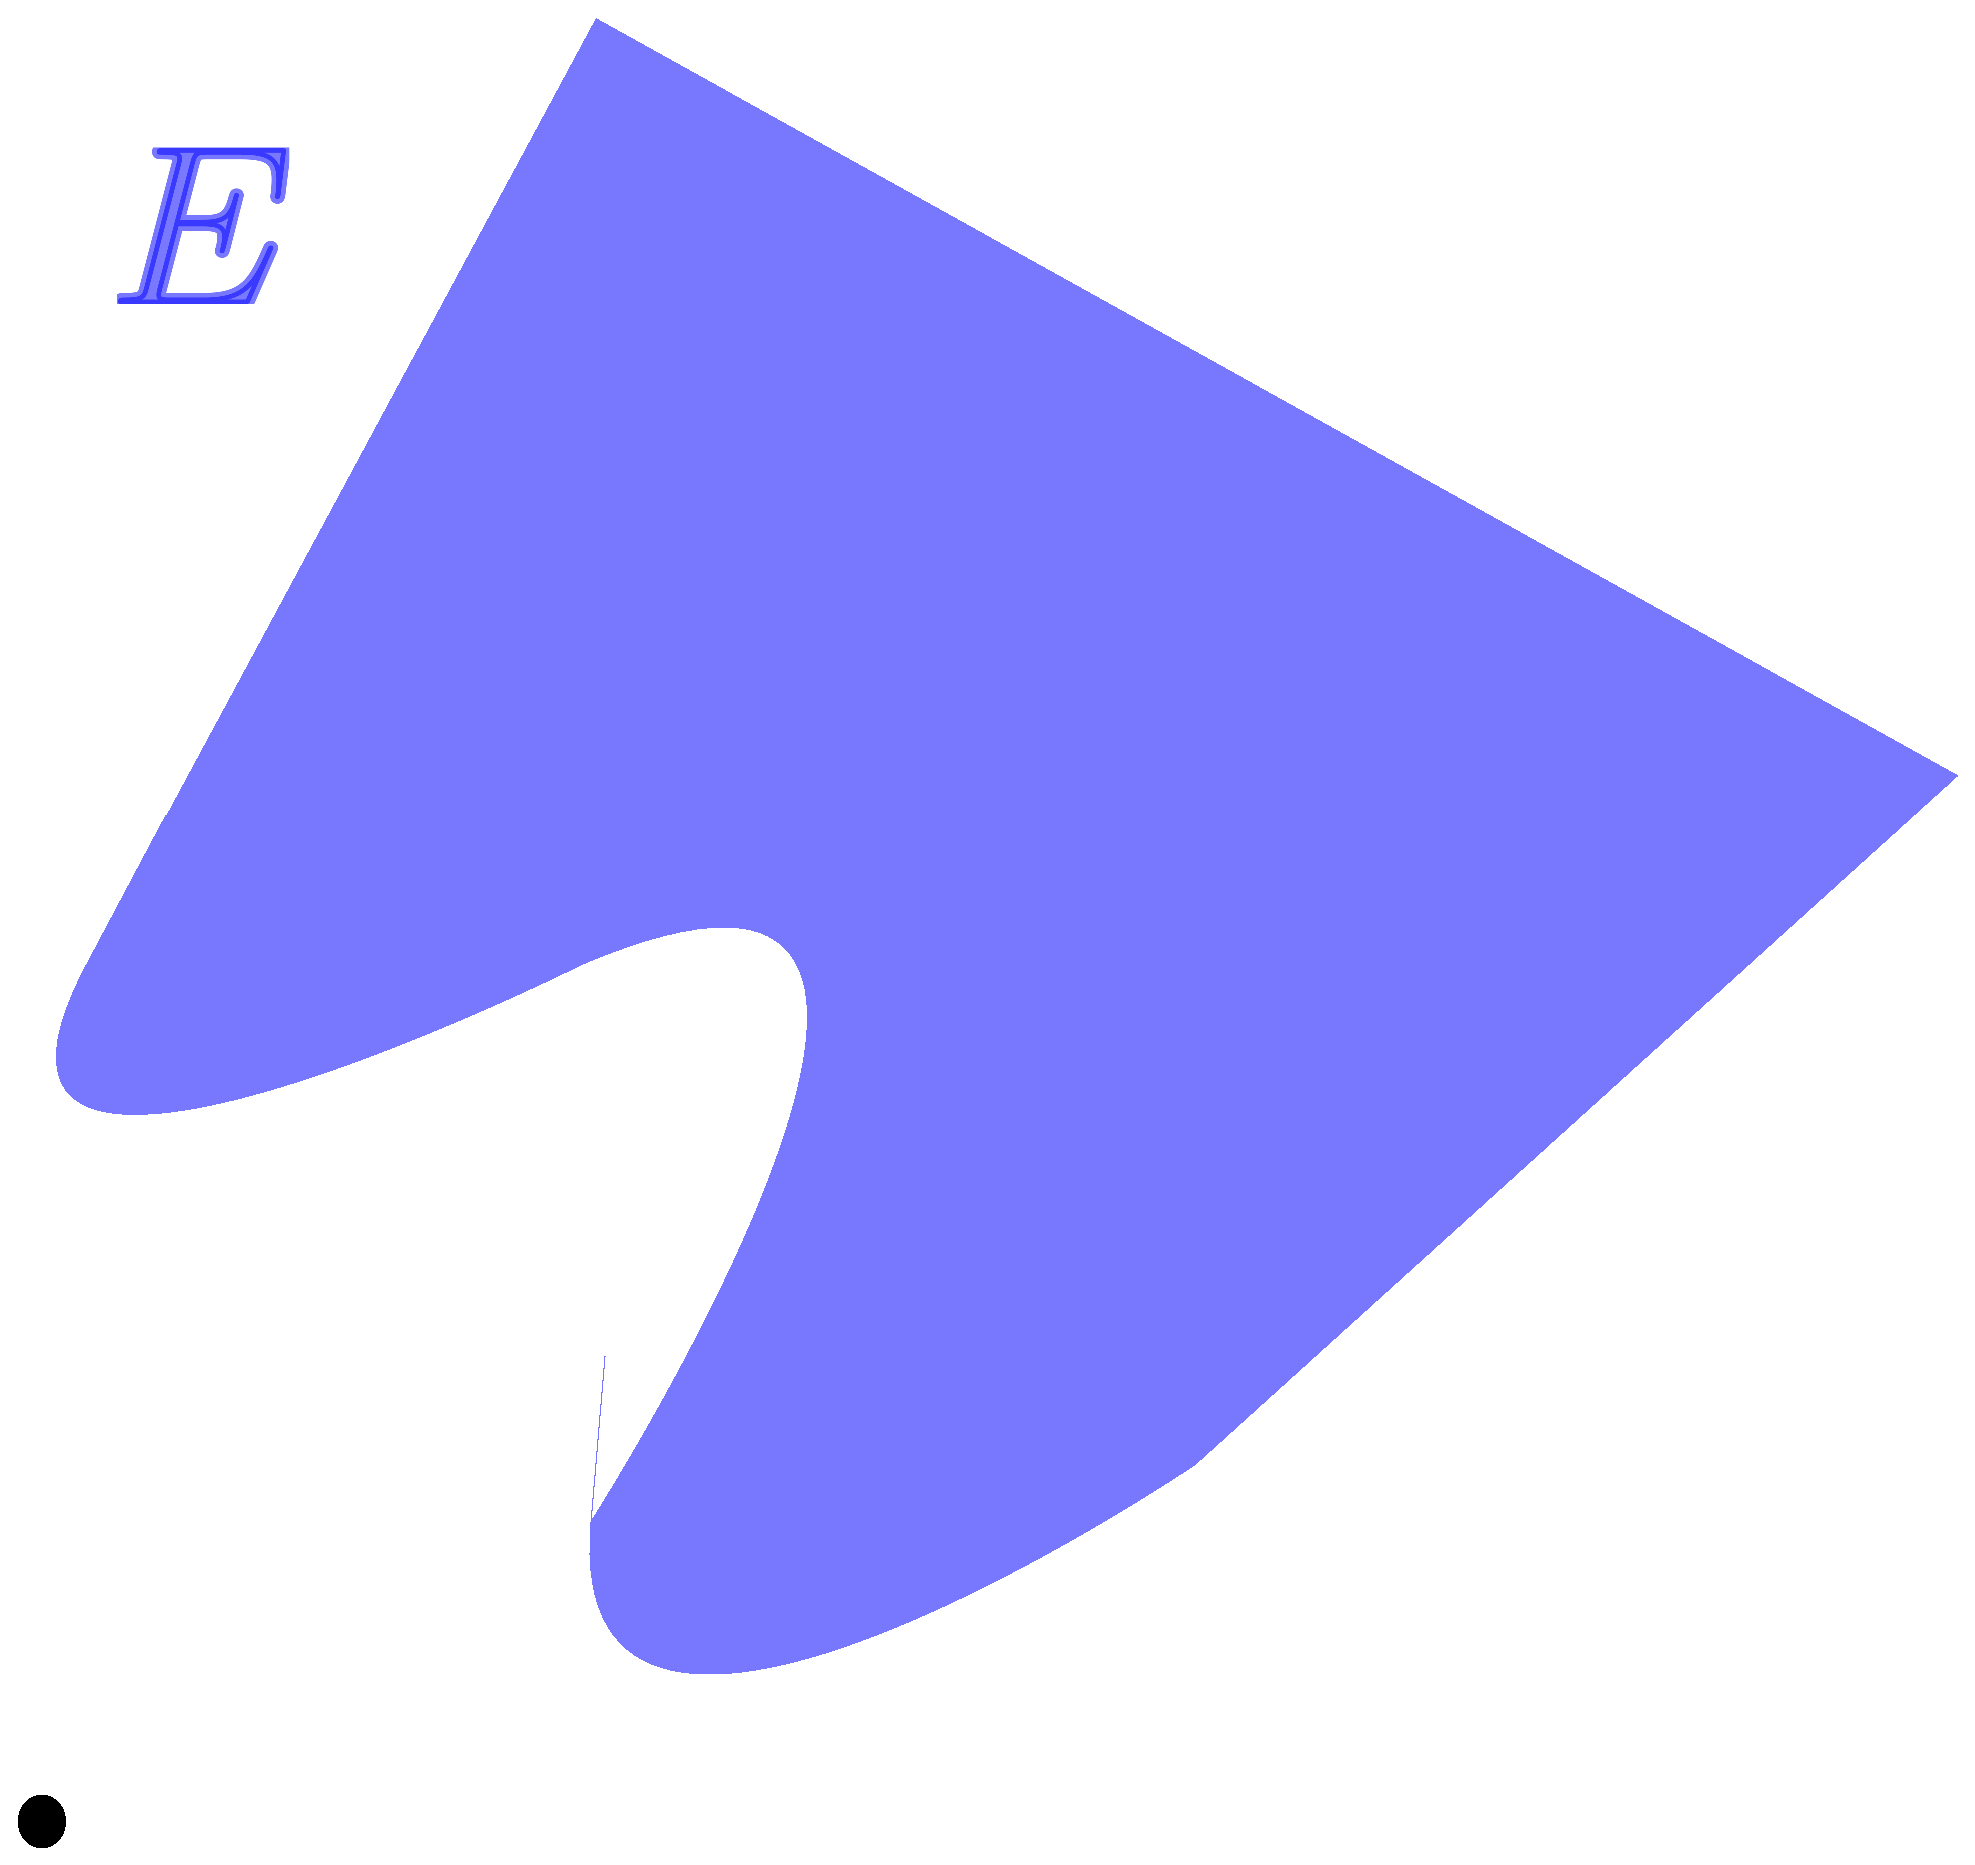
\includegraphics[keepaspectratio, scale=0.095]{figures/example_not_convex_asymptotically_regular_1.eps}
        \end{column}
        \pause
        \begin{column}{0.48\textwidth}
        \centering
        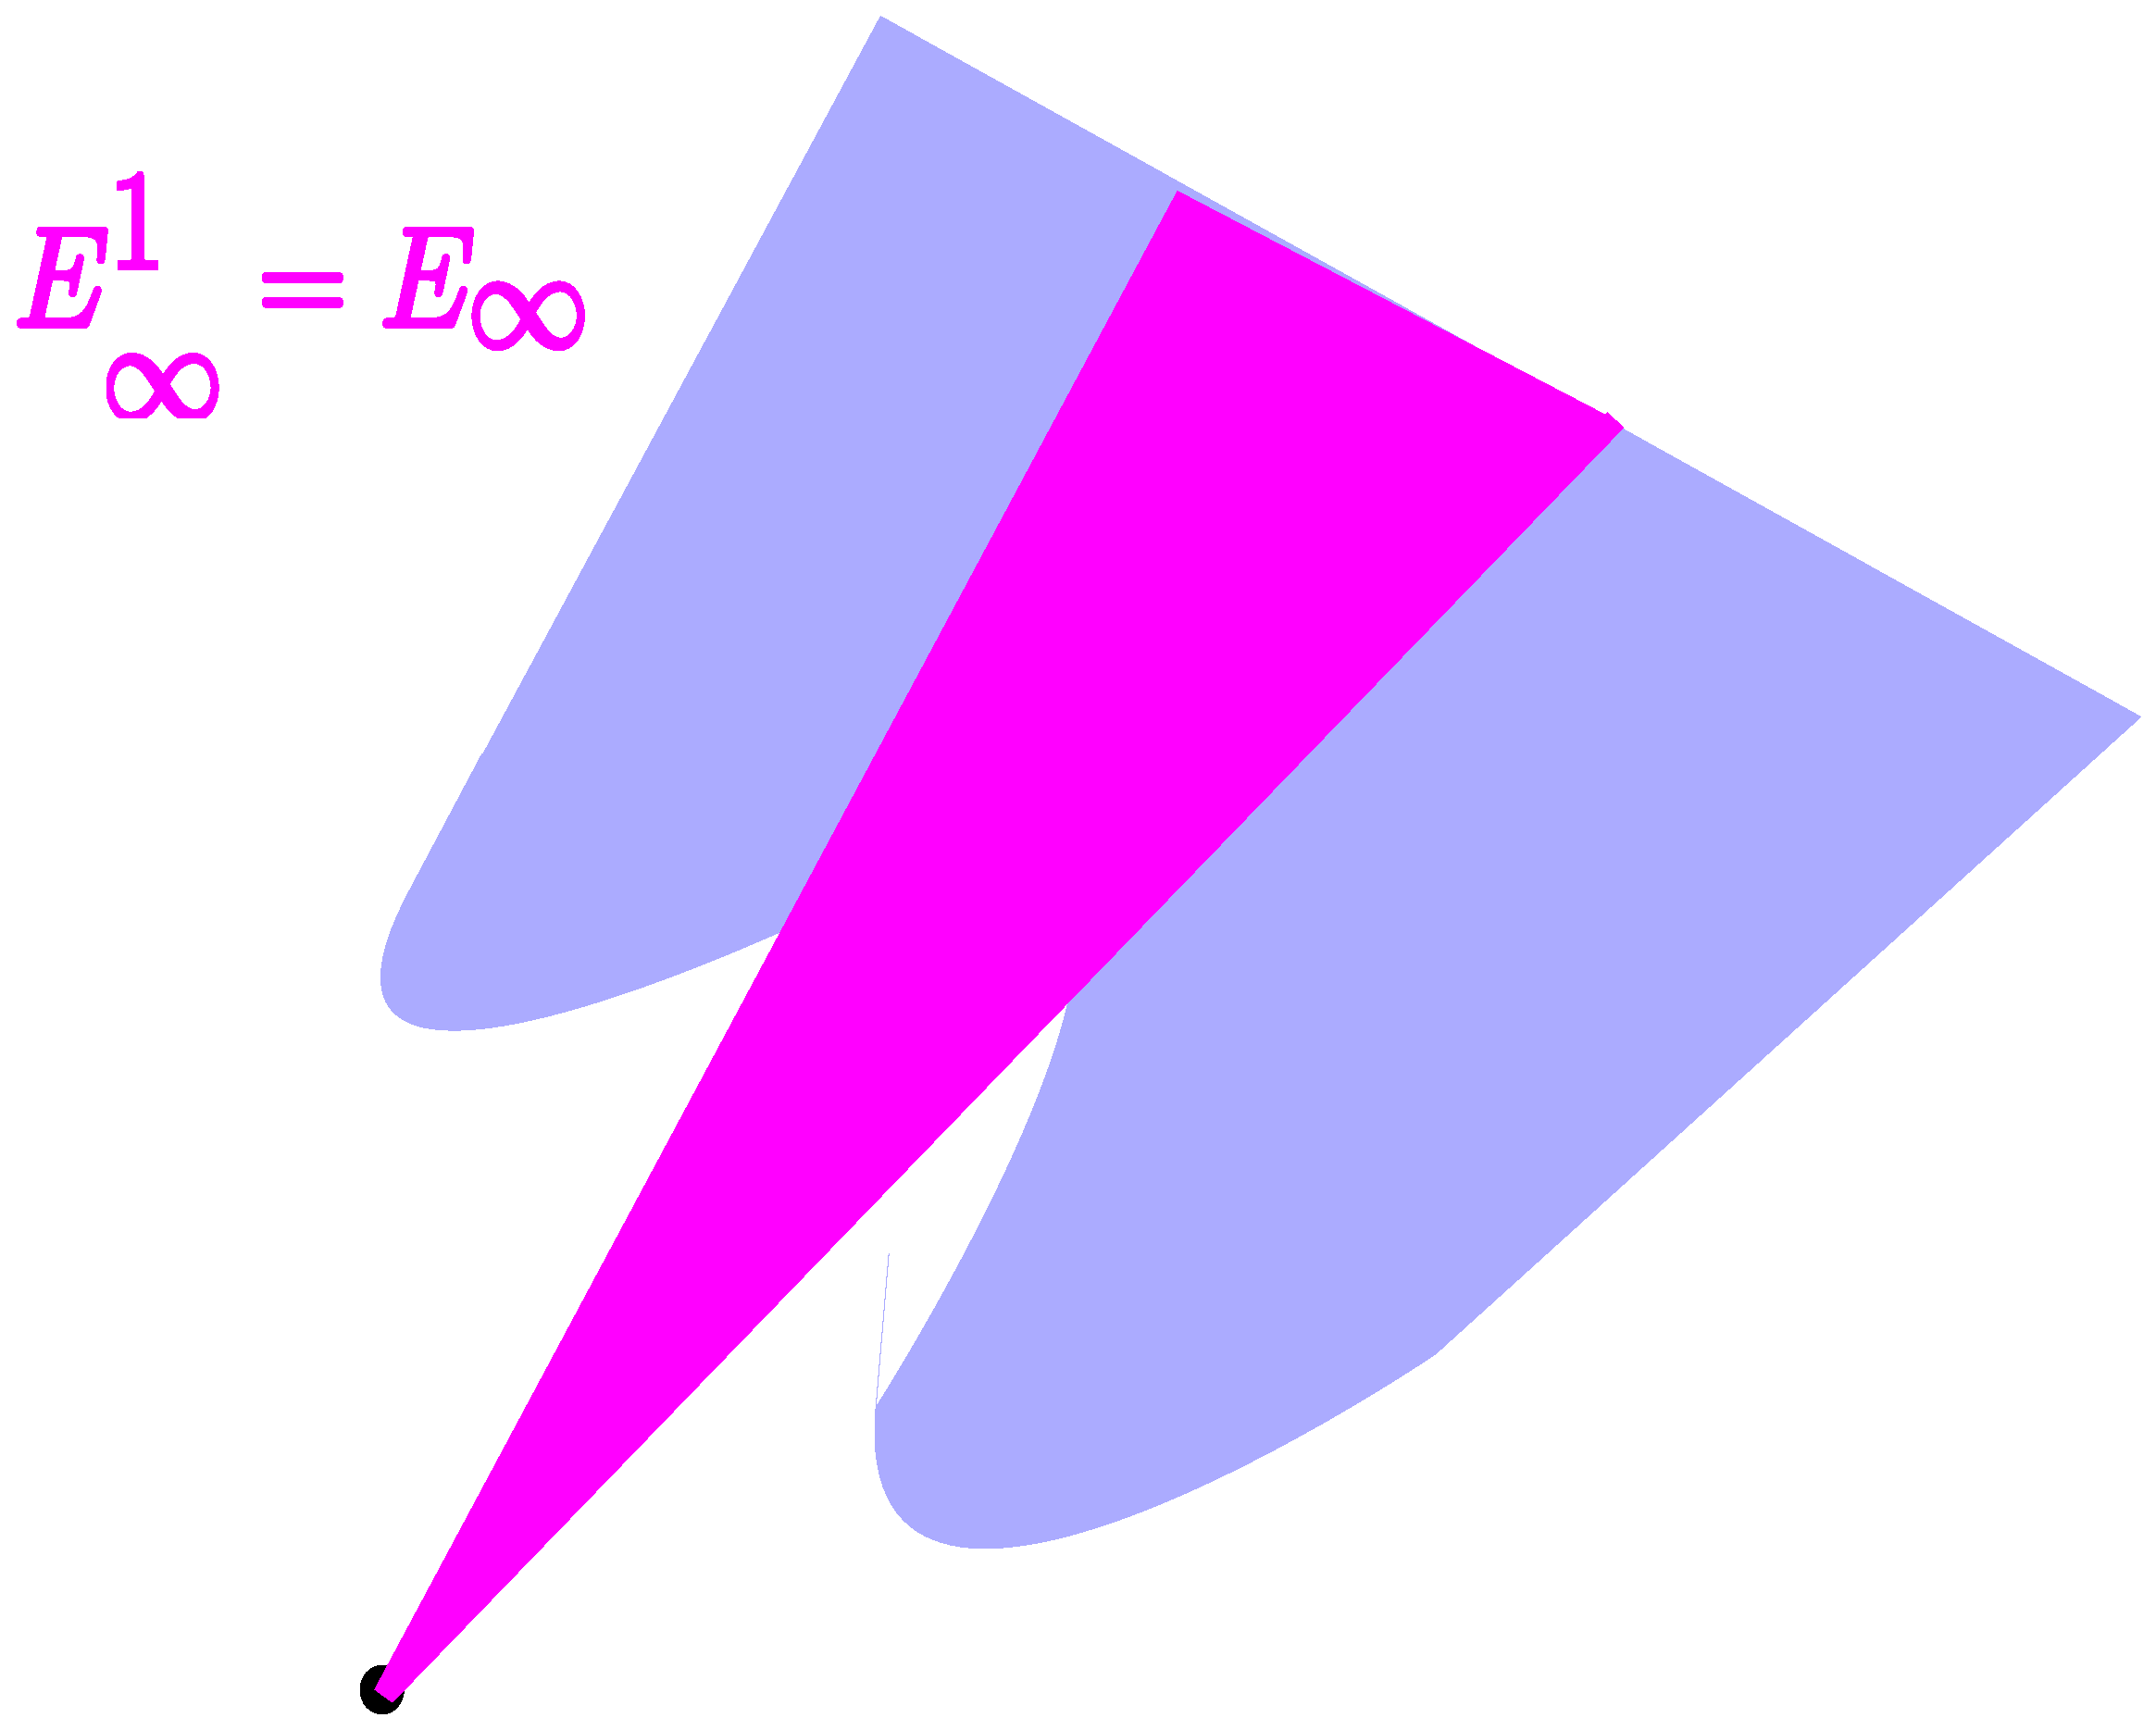
\includegraphics[keepaspectratio, scale=0.095]{figures/example_not_convex_asymptotically_regular_2.eps}
        \end{column}
    \end{columns}
\end{frame}

% 3.Painleve-Kuratowski Convergence
% ----------------------------------------------------------------
\section{\Painleve-Kuratowski Convergence}
\begin{frame}{Contents}
    \tableofcontents[currentsection]
\end{frame}

% 3.1
\begin{frame}{Definition of the \Painleve-Kuratowski Convergence}

    \begin{block}{Definition 4}
    $Y$: a topological vector space.

    $\mathcal{P}(Y)$: a family of subset in $Y$.

    Let $(A_n)_{n \in \NaturalNumberSet} \subset \mathcal{P}(Y)$. We define the inner limit and the outer limit as

    \begin{equation}
        \begin{split}
            \liminf_{n \to \infty}A_n &\coloneqq \SetForm{y \in Y}{\exists (y_n) \to y \SuchThat y_n \in A_n \:\text{for}\: n \geq n_0}, \\
            \limsup_{n \to \infty}A_n &\coloneqq \SetForm{y \in Y}{\exists (y_{n(k)}) \to y \SuchThat y_{n(k)} \in A_{n(k)} \:\text{for}\: k \in \NaturalNumberSet}. \notag
        \end{split}
    \end{equation}

    If it holds that $\liminf_{n \to \infty}A_n \supset \limsup_{n \to \infty}A_n$, we say that $(A_n)$ converges in the sense of \Painleve-Kuratowski.
    \end{block}
\end{frame}

% 3.2
\begin{frame}[t]{\Painleve-Kuratowski Convergence Examples}
Example:

\centering
\begin{columns}
    \begin{column}{0.48\textwidth}
    \centering
    \begin{equation}
        A_n = \begin{cases} [0, 1],  & \mbox{if }n\mbox{ is odd} \\ [0, \frac{1}{n}], & \mbox{if }n\mbox{ is even} \end{cases} \notag
    \end{equation}
    \end{column}
    \pause
    \begin{column}{0.48\textwidth}
    \centering
    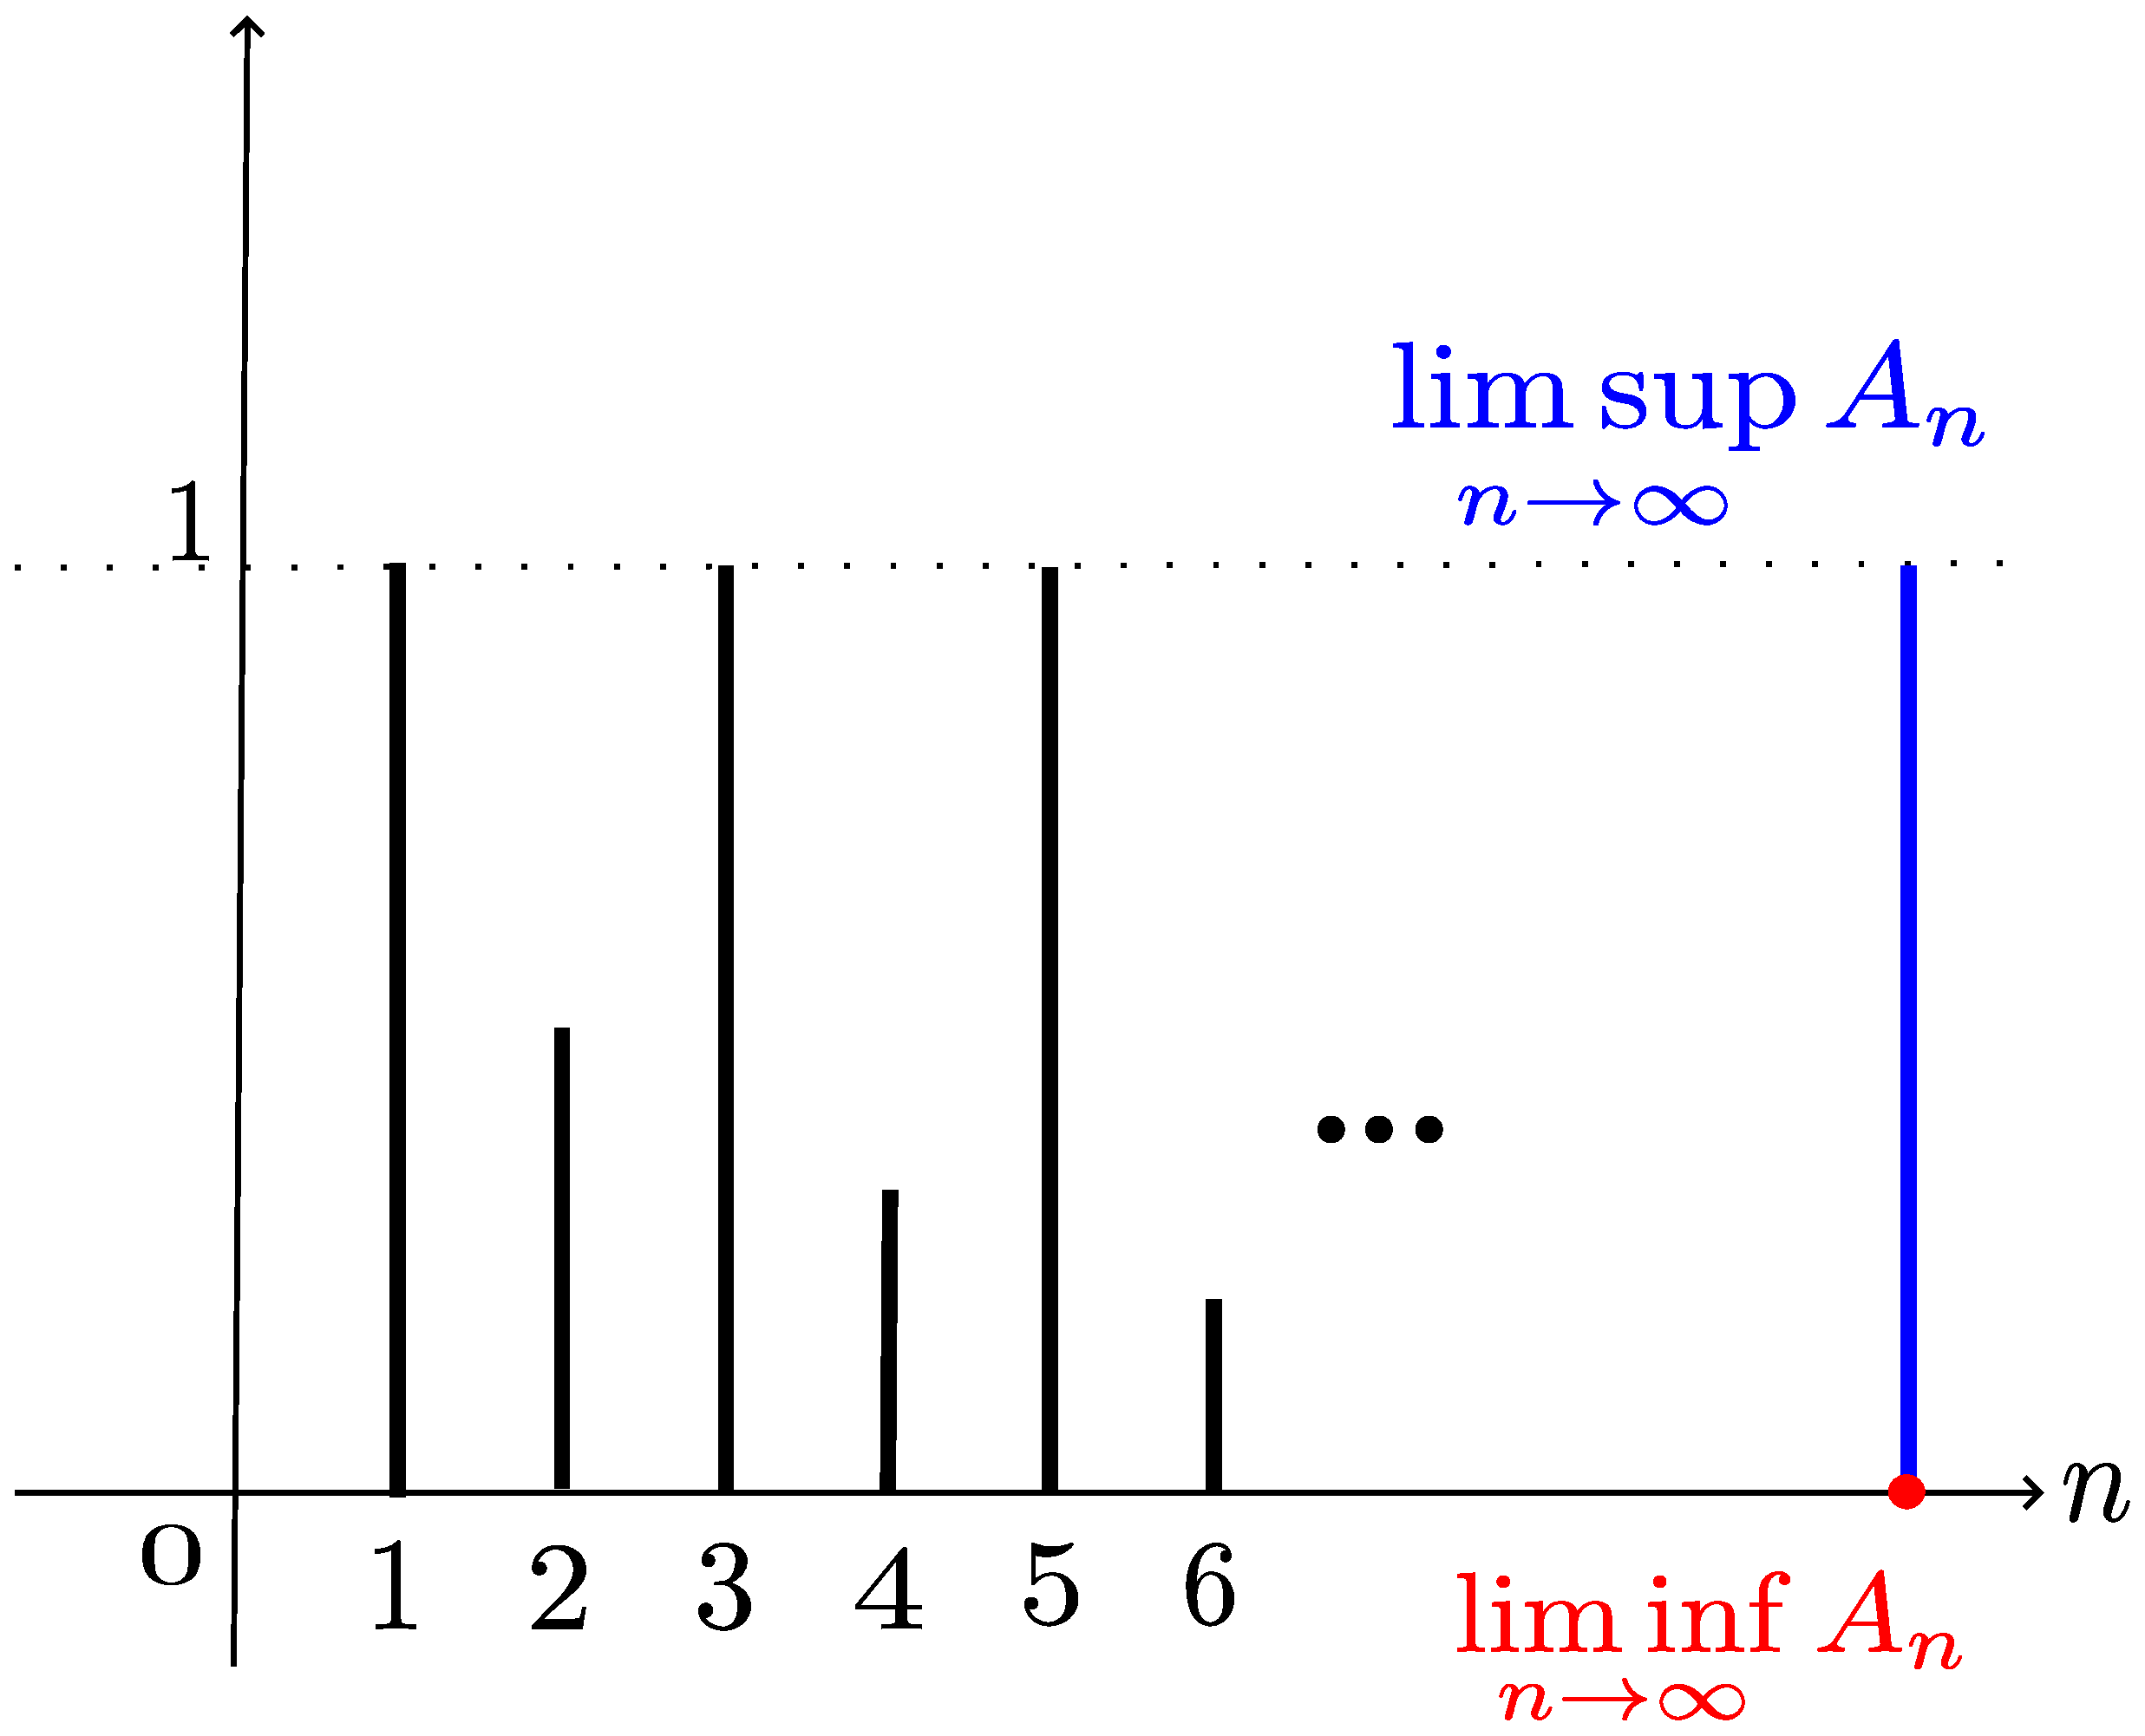
\includegraphics[keepaspectratio, scale=0.160]{figures/example_limsup_and_liminf.eps}
    \end{column}
\end{columns}
\end{frame}

% 3.3
\begin{frame}[t]{Relations between Asymptotic cones and \Painleve-Kuratowski Convergence}

\begin{alertblock}{Remark}
    Providing that the given $A_n$ converges in the sense of \Painleve-Kuratowski, we can let $\Gamma (n) = A_n$ and $\Gamma (\infty) = A$ where $A, A_n \subset Y$.
    Soon we can find that $\Gamma$ implies a set-valued mapping.
\end{alertblock}

\begin{columns}
    \begin{column}{0.48\textwidth}
    $C$: a nonempty set

    $\Gamma$: $\NaturalNumberSet \rightarrow \NDemenstionalRealEuclideanSpace$

    We let $\Gamma (n) = \frac{C}{n}$.

    \pause
    \centering
    \begin{equation}
        \begin{split}
            \liminf_{n \to \infty} \frac{C}{n} &= C^1_{\infty} \\
            \limsup_{n \to \infty}\frac{C}{n} &= C_{\infty} \\
            \Gamma (\infty) &= C^1_{\infty} = C_{\infty} \text{ (if $\{C_n\}_{n \in \NaturalNumberSet} \coloneqq \frac{C}{n}$ converges in the sense of \Painleve-Kuratowski)} \notag
        \end{split}
    \end{equation}
    \end{column}
    \pause
    \begin{column}{0.48\textwidth}
    \centering
    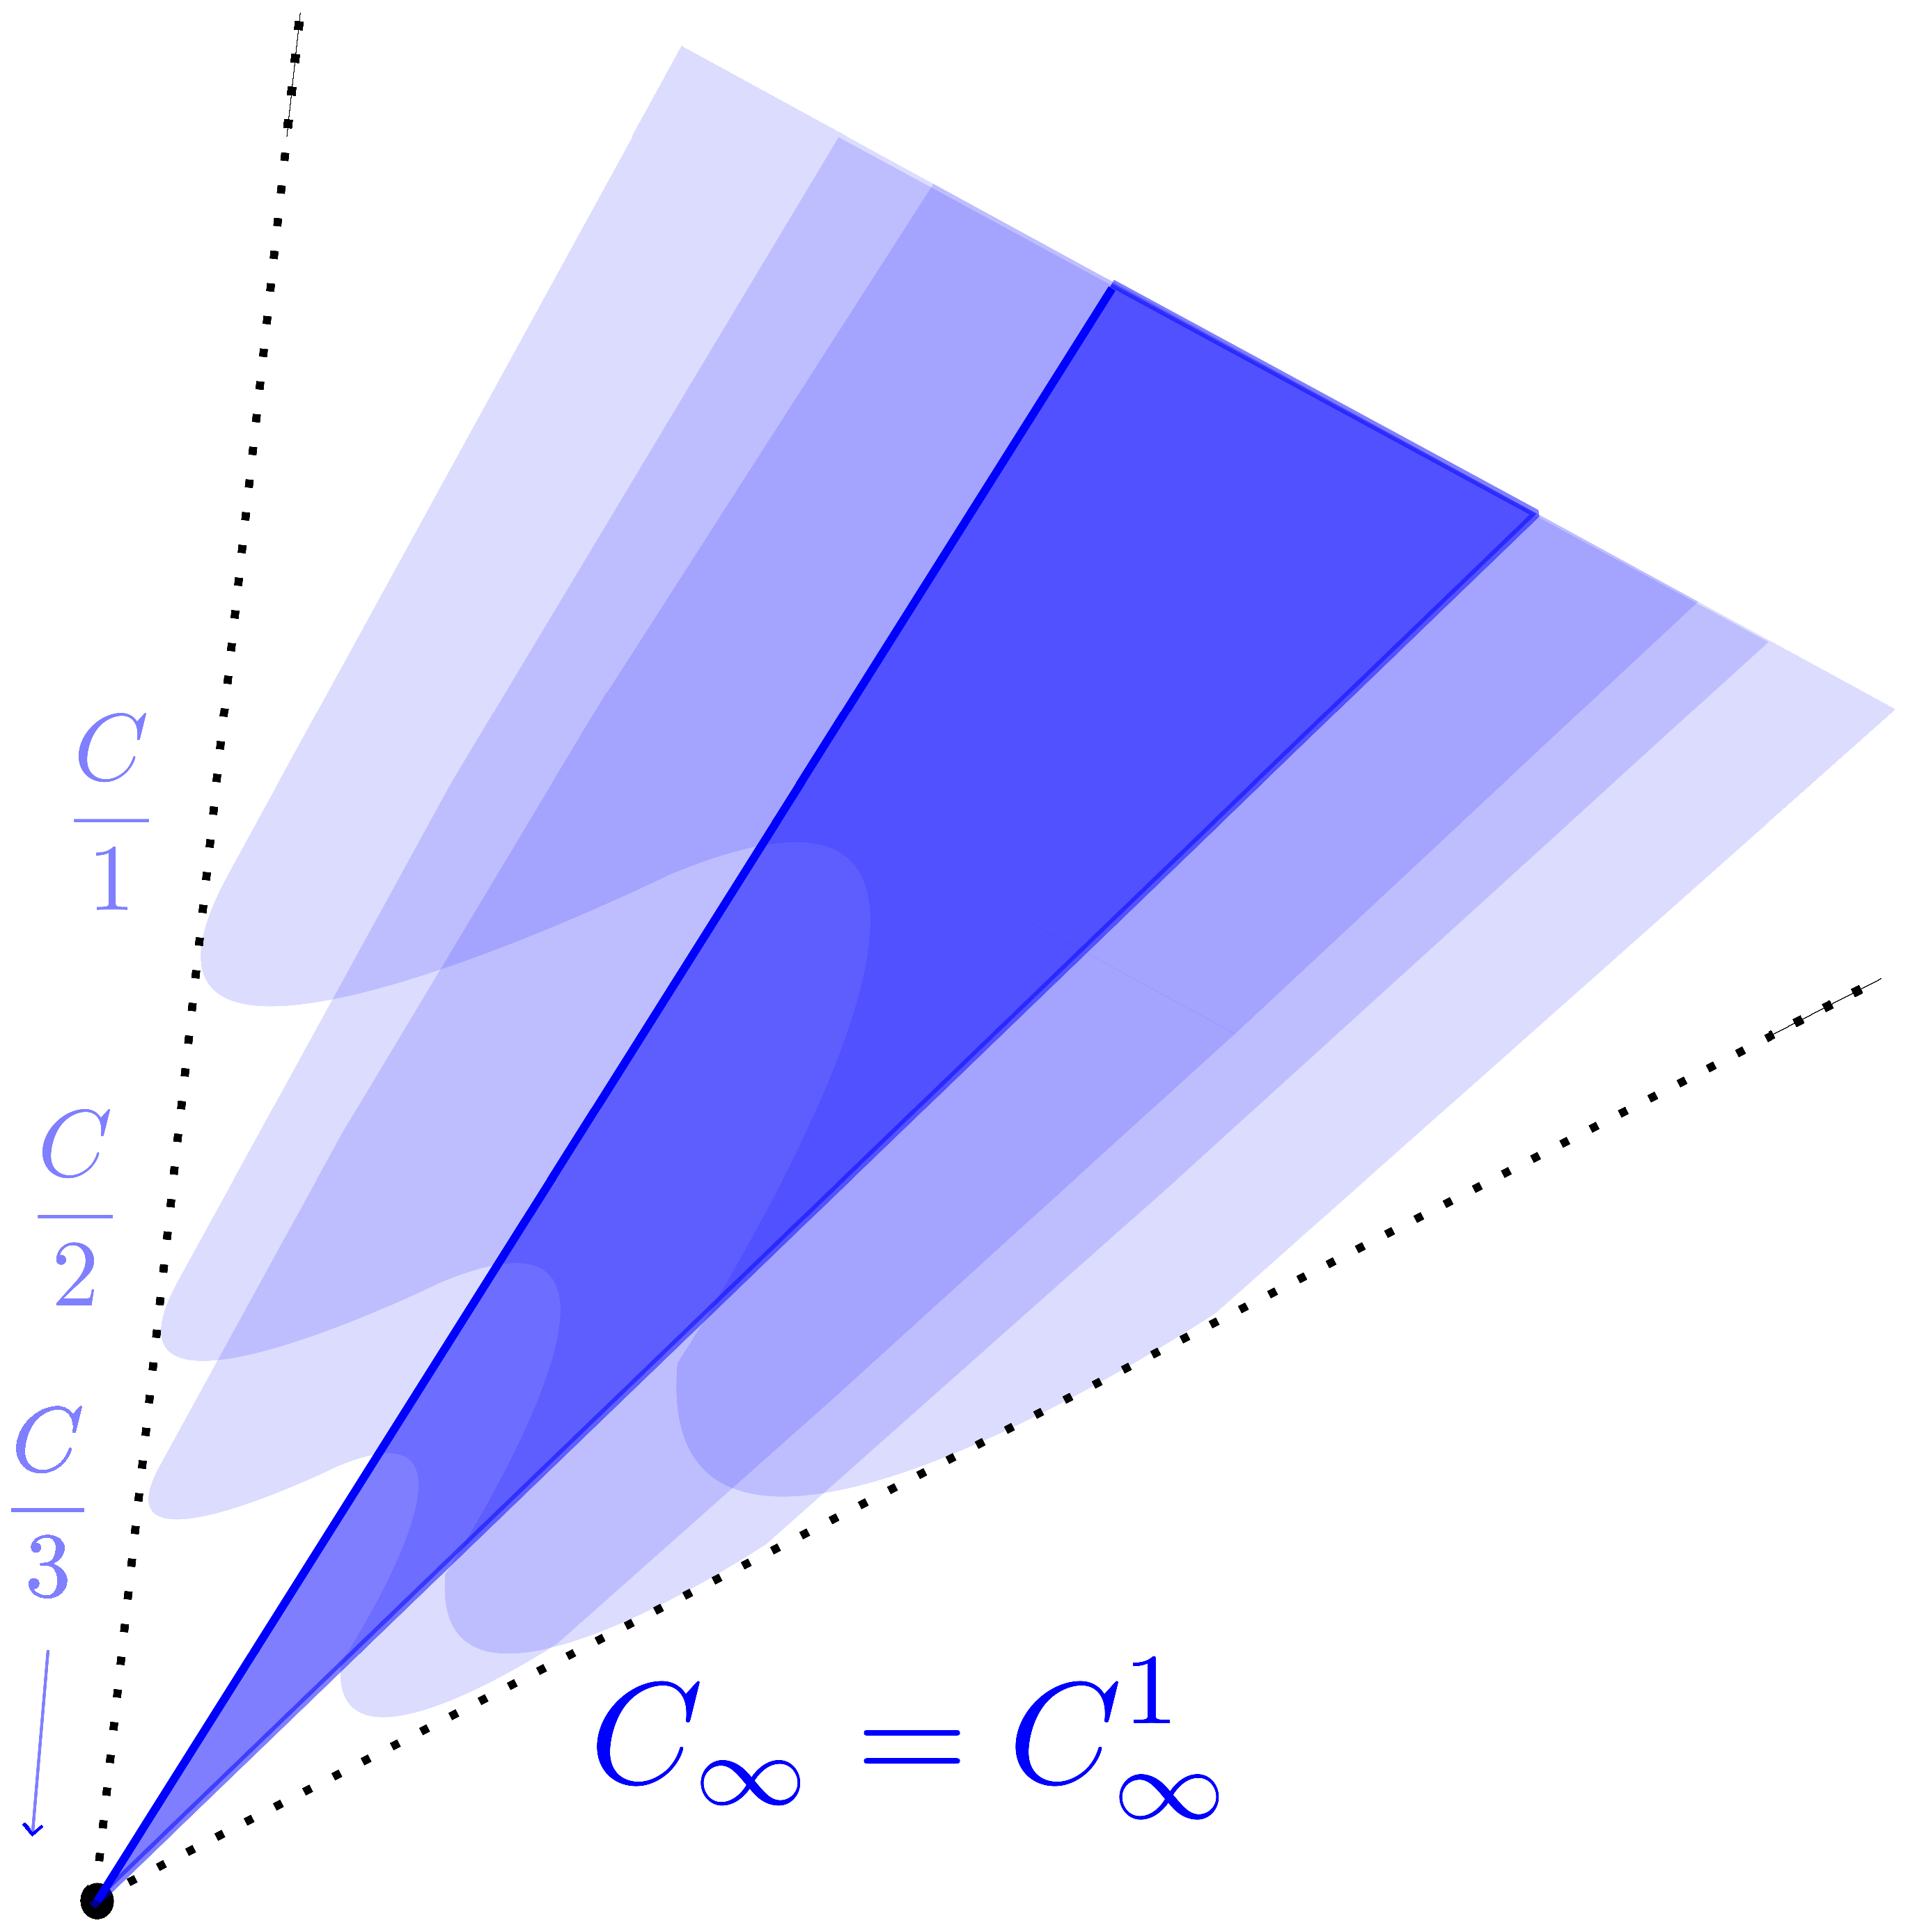
\includegraphics[keepaspectratio, scale=0.08]{figures/relation_asymptotice_cone_and_p_k_convergence.eps}
    \end{column}
\end{columns}
\end{frame}

% 4.Conclusions
% ----------------------------------------------------------------
\section{Conclusions}
\begin{frame}{Contents}
    \tableofcontents[currentsection]
\end{frame}

% 3.1
\begin{frame}{Conclusions}
    \begin{enumerate}[]
        \item Considering a set-valued mappings, we can replace the definition of asymptotic cones as the inner limit.
        \item The relation allows us to connect the notion of asymptotic cones with some results of continuities in t.v.s.
    \end{enumerate}
\end{frame}

% 4.References
% ----------------------------------------------------------------
\begin{frame}[t]{References}
\begin{enumerate}[]
    \item A. G\"{o}pfert, H. Riahi, C. Tammer, and C. Z\u{a}linescu, Variational methods in partially ordered spaces, vol. 17 of CMS Books in Mathematics, Springer-Verlag, New York, 2003.
    \item A. Alfred and M. Teboulle, asymptotic cones and functions in optimization and variational inequalities, Springer monographs in Mathematics, Springer-Verlag, New York, 2003.
\end{enumerate}
\end{frame}

\end{document}
